% 若编译失败,且生成 .synctex(busy) 辅助文件,可能有两个原因:
% 1. 需要插入的图片不存在:Ctrl + F 搜索 'figure' 将这些代码注释/删除掉即可
% 2. 路径/文件名含中文或空格:更改路径/文件名即可

% --------------------- 文章宏包及相关设置 --------------------- %
% >> ------------------ 文章宏包及相关设置 ------------------ << %
% 设定文章类型与编码格式
    \documentclass[UTF8]{report}		

% 本 .tex 专属的宏定义
    \def\V{\ \mathrm{V}}
    \def\mV{\ \mathrm{mV}}
    \def\kV{\ \mathrm{KV}}
    \def\KV{\ \mathrm{KV}}
    \def\MV{\ \mathrm{MV}}
    \def\A{\ \mathrm{A}}
    \def\mA{\ \mathrm{mA}}
    \def\kA{\ \mathrm{KA}}
    \def\KA{\ \mathrm{KA}}
    \def\MA{\ \mathrm{MA}}
    \def\O{\ \Omega}
    \def\mO{\ \Omega}
    \def\kO{\ \mathrm{K}\Omega}
    \def\KO{\ \mathrm{K}\Omega}
    \def\MO{\ \mathrm{M}\Omega}
    \def\Hz{\ \mathrm{Hz}}

% 自定义宏定义
    \def\N{\mathbb{N}}
    \def\F{\mathbb{F}}
    \def\Z{\mathbb{Z}}
    \def\Q{\mathbb{Q}}
    \def\R{\mathbb{R}}
    \def\C{\mathbb{C}}
    \def\T{\mathbb{T}}
    \def\S{\mathbb{S}}
    \def\A{\mathbb{A}}
    \def\I{\mathscr{I}}
    \def\Im{\mathrm{Im\,}}
    \def\Re{\mathrm{Re\,}}
    \def\d{\mathrm{d}}
    \def\p{\partial}

% 导入基本宏包
    \usepackage[UTF8]{ctex}     % 设置文档为中文语言
        \usepackage{hyperref}  % 宏包:自动生成超链接 (此宏包与标题中的数学环境冲突)
    \hypersetup{
        colorlinks=true,    % false:边框链接 ; true:彩色链接
        citecolor={blue},    % 文献引用颜色
        linkcolor={blue},   % 目录 (我们在目录处单独设置),公式,图表,脚注等内部链接颜色
        urlcolor={magenta},    % 网页 URL 链接颜色,包括 \href 中的 text
        % cyan 浅蓝色 
        % magenta 洋红色
        % yellow 黄色
        % black 黑色
        % white 白色
        % red 红色
        % green 绿色
        % blue 蓝色
        % gray 灰色
        % darkgray 深灰色
        % lightgray 浅灰色
        % brown 棕色
        % lime 石灰色
        % olive 橄榄色
        % orange 橙色
        % pink 粉红色
        % purple 紫色
        % teal 蓝绿色
        % violet 紫罗兰色
    }
    % \usepackage{docmute}    % 宏包:子文件导入时自动去除导言区,用于主/子文件的写作方式,\include{./51单片机笔记}即可。注:启用此宏包会导致.tex文件capacity受限。
    \usepackage{amsmath}    % 宏包:数学公式
    \usepackage{mathrsfs}   % 宏包:提供更多数学符号
    \usepackage{amssymb}    % 宏包:提供更多数学符号
    \usepackage{pifont}     % 宏包:提供了特殊符号和字体
    \usepackage{extarrows}  % 宏包:更多箭头符号


% 文章页面margin设置
    \usepackage[a4paper]{geometry}
        \geometry{top=1in}
        \geometry{bottom=1in}
        \geometry{left=0.75in}
        \geometry{right=0.75in}   % 设置上下左右页边距
        \geometry{marginparwidth=1.75cm}    % 设置边注距离(注释、标记等)

% 配置数学环境
    \usepackage{amsthm} % 宏包:数学环境配置
    %\everymath{\displaystyle}   % 设置全文数学公式都为展示样式
    % theorem-line 环境自定义
        \newtheoremstyle{MyLineTheoremStyle}% <name>
            {11pt}% <space above>
            {11pt}% <space below>
            {\kaishu}% <body font> 使用默认正文字体
            {}% <indent amount>
            {\bfseries}% <theorem head font> 设置标题项为加粗
            {:}% <punctuation after theorem head>
            {.5em}% <space after theorem head>
            {\textbf{#1}\thmnumber{#2}\ \ (\,\textbf{#3}\,)}% 设置标题内容顺序
        \theoremstyle{MyLineTheoremStyle} % 应用自定义的定理样式
        \newtheorem{LineTheorem}{Theorem.\,}
    % theorem-block 环境自定义
        \newtheoremstyle{MyBlockTheoremStyle}% <name>
            {11pt}% <space above>
            {11pt}% <space below>
            {\kaishu}% <body font> 使用默认正文字体
            {}% <indent amount>
            {\bfseries}% <theorem head font> 设置标题项为加粗
            {:\\ \indent}% <punctuation after theorem head>
            {.5em}% <space after theorem head>
            {\textbf{#1}\thmnumber{#2}\ \ (\,\textbf{#3}\,)}% 设置标题内容顺序
        \theoremstyle{MyBlockTheoremStyle} % 应用自定义的定理样式
        \newtheorem{BlockTheorem}[LineTheorem]{Theorem.\,} % 使用 LineTheorem 的计数器
    % definition 环境自定义
        \newtheoremstyle{MySubsubsectionStyle}% <name>
            {11pt}% <space above>
            {11pt}% <space below>
            {}% <body font> 使用默认正文字体
            {}% <indent amount>
            {\bfseries}% <theorem head font> 设置标题项为加粗
            {:\\ \indent}% <punctuation after theorem head>
            {0pt}% <space after theorem head>
            {\textbf{#3}}% 设置标题内容顺序
        \theoremstyle{MySubsubsectionStyle} % 应用自定义的定理样式
        \newtheorem{definition}{}

%宏包:有色文本框(proof环境)及其设置
    \usepackage[dvipsnames,svgnames]{xcolor}    %设置插入的文本框颜色
    \usepackage[strict]{changepage}     % 提供一个 adjustwidth 环境
    \usepackage{framed}     % 实现方框效果
        \definecolor{graybox_color}{rgb}{0.95,0.95,0.96} % 文本框颜色。修改此行中的 rgb 数值即可改变方框纹颜色,具体颜色的rgb数值可以在网站https://colordrop.io/ 中获得。(截止目前的尝试还没有成功过,感觉单位不一样)(找到喜欢的颜色,点击下方的小眼睛,找到rgb值,复制修改即可)
        \newenvironment{graybox}{%
        \def\FrameCommand{%
        \hspace{1pt}%
        {\color{gray}\small \vrule width 2pt}%
        {\color{graybox_color}\vrule width 4pt}%
        \colorbox{graybox_color}%
        }%
        \MakeFramed{\advance\hsize-\width\FrameRestore}%
        \noindent\hspace{-4.55pt}% disable indenting first paragraph
        \begin{adjustwidth}{}{7pt}%
        \vspace{2pt}\vspace{2pt}%
        }
        {%
        \vspace{2pt}\end{adjustwidth}\endMakeFramed%
        }

% 外源代码插入设置
    % matlab 代码插入设置
    \usepackage{matlab-prettifier}
        \lstset{style=Matlab-editor}    % 继承 matlab 代码高亮 , 此行不能删去
    \usepackage[most]{tcolorbox} % 引入tcolorbox包 
    \usepackage{listings} % 引入listings包
        \tcbuselibrary{listings, skins, breakable}
        \newfontfamily\codefont{Consolas} % 定义需要的 codefont 字体
        \lstdefinestyle{MatlabStyle_inc}{   % 插入代码的样式
            language=Matlab,
            basicstyle=\small\ttfamily\codefont,    % ttfamily 确保等宽 
            breakatwhitespace=false,
            breaklines=true,
            captionpos=b,
            keepspaces=true,
            numbers=left,
            numbersep=15pt,
            showspaces=false,
            showstringspaces=false,
            showtabs=false,
            tabsize=2,
            xleftmargin=15pt,   % 左边距
            %frame=single, % single 为包围式单线框
            frame=shadowbox,    % shadowbox 为带阴影包围式单线框效果
            %escapeinside=``,   % 允许在代码块中使用 LaTeX 命令 (此行无用)
            %frameround=tttt,    % tttt 表示四个角都是圆角
            framextopmargin=0pt,    % 边框上边距
            framexbottommargin=0pt, % 边框下边距
            framexleftmargin=5pt,   % 边框左边距
            framexrightmargin=5pt,  % 边框右边距
            rulesepcolor=\color{red!20!green!20!blue!20}, % 阴影框颜色设置
            %backgroundcolor=\color{blue!10}, % 背景颜色
        }
        \lstdefinestyle{MatlabStyle_src}{   % 插入代码的样式
            language=Matlab,
            basicstyle=\small\ttfamily\codefont,    % ttfamily 确保等宽 
            breakatwhitespace=false,
            breaklines=true,
            captionpos=b,
            keepspaces=true,
            numbers=left,
            numbersep=15pt,
            showspaces=false,
            showstringspaces=false,
            showtabs=false,
            tabsize=2,
        }
        \newtcblisting{matlablisting}{
            %arc=2pt,        % 圆角半径
            % 调整代码在 listing 中的位置以和引入文件时的格式相同
            top=0pt,
            bottom=0pt,
            left=-5pt,
            right=-5pt,
            listing only,   % 此句不能删去
            listing style=MatlabStyle_src,
            breakable,
            colback=white,   % 选一个合适的颜色
            colframe=black!0,   % 感叹号后跟不透明度 (为 0 时完全透明)
        }
        \lstset{
            style=MatlabStyle_inc,
        }

% table 支持
    \usepackage{booktabs}   % 宏包:三线表
    \usepackage{tabularray} % 宏包:表格排版
    \usepackage[longtable]{multirow} % 宏包:multi 行列
    \usepackage{longtable}  % 宏包:长表格

% figure 设置
    \usepackage{graphicx}  % 支持 jpg, png, eps, pdf 图片 
    \usepackage{svg}       % 支持 svg 图片
        \svgsetup{
            % 指向 inkscape.exe 的路径
            inkscapeexe = C:/aa_MySame/inkscape/bin/inkscape.exe, 
            % 一定程度上修复导入后图片文字溢出几何图形的问题
            inkscapelatex = false                 
        }
    \usepackage{subcaption} % 支持子图

% 图表进阶设置
    \usepackage{caption}    % 图注、表注
        \captionsetup[figure]{name=图}  
        \captionsetup[table]{name=表}
        \captionsetup{labelfont=bf, font=small}
    \usepackage{float}     % 图表位置浮动设置 

% 圆圈序号自定义
    \newcommand*\circled[1]{\tikz[baseline=(char.base)]{\node[shape=circle,draw,inner sep=0.8pt, line width = 0.03em] (char) {\small \bfseries #1};}}   % TikZ solution

% 列表设置
    \usepackage{enumitem}   % 宏包:列表环境设置
        \setlist[enumerate]{itemsep=0pt, parsep=0pt, topsep=0pt, partopsep=0pt, leftmargin=3.5em} 
        \setlist[itemize]{itemsep=0pt, parsep=0pt, topsep=0pt, partopsep=0pt, leftmargin=3.5em}
        \newlist{circledenum}{enumerate}{1} % 创建一个新的枚举环境  
        \setlist[circledenum,1]{  
            label=\protect\circled{\arabic*}, % 使用 \arabic* 来获取当前枚举计数器的值,并用 \circled 包装它  
            ref=\arabic*, % 如果需要引用列表项,这将决定引用格式(这里仍然使用数字)
            itemsep=0pt, parsep=0pt, topsep=0pt, partopsep=0pt, leftmargin=3.5em
        }  
    

% 文章默认字体设置
    \usepackage{fontspec}   % 宏包:字体设置
        \setmainfont{SimSun}    % 设置中文字体为宋体字体
        \setCJKmainfont[AutoFakeBold=3]{SimSun} % 设置加粗字体为 SimSun 族,AutoFakeBold 可以调整字体粗细
        \setmainfont{Times New Roman} % 设置英文字体为Times New Roman


% 文章序言设置
    \newcommand{\cnabstractname}{序言}
    \newenvironment{cnabstract}{%
        \par\Large
        \noindent\mbox{}\hfill{\bfseries \cnabstractname}\hfill\mbox{}\par
        \vskip 2.5ex
        }{\par\vskip 2.5ex}

% 参考文献引用设置
    \bibliographystyle{unsrt}   % 设置参考文献引用格式为unsrt
    \newcommand{\upcite}[1]{\textsuperscript{\cite{#1}}}     % 自定义上角标式引用

% 各级标题自定义设置
    \usepackage{titlesec}   
    % chapter
        \titleformat{\chapter}[hang]{\normalfont\Large\bfseries\centering\boldmath}{}{10pt}{}
        %\titleformat{\chapter}[hang]{\normalfont\Large\bfseries\centering\boldmath}{Homework \thechapter :}{10pt}{}
        \titlespacing*{\chapter}{0pt}{-30pt}{10pt} % 控制上方空白的大小
    % section
        \titleformat{\section}[hang]{\normalfont\large\bfseries\boldmath}{\thesection}{8pt}{}
    % subsection
        % 设置 subsection 样式为 (1) (2) (3)
        \renewcommand{\thesubsection}{(\arabic{subsection})}    
        \titleformat{\subsection}[hang]{\normalfont\bfseries\boldmath}{\thesubsection}{8pt}{}


% --------------------- 文章宏包及相关设置 --------------------- %
% >> ------------------ 文章宏包及相关设置 ------------------ << %



% ------------------------ 文章信息区 ------------------------ %
% >> --------------------- 文章信息区 --------------------- << %
% 页眉页脚设置
\usepackage{fancyhdr}   %宏包:页眉页脚设置
    \pagestyle{fancy}
    \fancyhf{}
    \cfoot{\thepage}
    \renewcommand\headrulewidth{1pt}
    \renewcommand\footrulewidth{0pt}
    \chead{电路原理课程作业,\ 丁毅,\ 2023K8009908031}
    \lhead{Homework \thechapter}
    \rhead{dingyi233@mails.ucas.ac.cn}

%文档信息设置
\title{电路原理课程作业\\ Homework of Principles of Electric Circuits }
\author{丁毅\\ \footnotesize 中国科学院大学,北京 100049\\ Yi Ding \\ \footnotesize University of Chinese Academy of Sciences, Beijing 100049, China}
\date{\footnotesize 2024.8 -- 2025.1}
% >> --------------------- 文章信息区 --------------------- << %
% ------------------------ 文章信息区 ------------------------ %

% 开始编辑文章

\begin{document}
\zihao{5}           % 设置全文字号大小

% ------------------------ 封面序言与目录 ------------------------ %
% >> --------------------- 封面序言与目录 --------------------- << %
% 封面
    \maketitle\newpage  
    \pagenumbering{Roman} % 页码为大写罗马数字
    \thispagestyle{fancy}   % 显示页码、页眉等

% 序言
    \begin{cnabstract}\normalsize 
        本文为笔者本科时的“电路原理”课程作业(Homework of Principles of Electric Circuits, 2024.9-2025.1)。由于个人学识浅陋,认识有限,文中难免有不妥甚至错误之处,望读者不吝指正,在此感谢。\par 
        我的邮箱是 dingyi233@mails.ucas.ac.cn。
    \end{cnabstract}
    \addcontentsline{toc}{chapter}{序言} % 手动添加为目录

% 不换页目录
    \setcounter{tocdepth}{0}
    \noindent\rule{\textwidth}{0.1em}   % 分割线
    \noindent\begin{minipage}{\textwidth}\centering 
        \vspace{1cm}
        \tableofcontents\thispagestyle{fancy}   % 显示页码、页眉等   
    \end{minipage}  
    \addcontentsline{toc}{chapter}{目录} % 手动添加为目录

% 收尾工作
    \newpage    
    \pagenumbering{arabic} 

% >> --------------------- 封面序言与目录 --------------------- << %
% ------------------------ 封面序言与目录 ------------------------ %

\chapter{Homework 1: 2024.8.27 - 2024.9.2}\thispagestyle{fancy}

\section{习题集 1-2: 求题图各电路中的电压 $U$ 和电流 $I$}

\begin{enumerate}
\item[(a)] 短路,因此 $U = 0,\  I = \frac{U_S}{R_i}$
\item[(b)] 开路,因此 $U = U_s, \ I = 0$
\item[(c)] 构成回路,因此  $ U = \frac{U_SR}{R + R_i},\ I = \frac{U_S}{R + R_i}$ 
\end{enumerate}

\begin{figure}[H]\centering
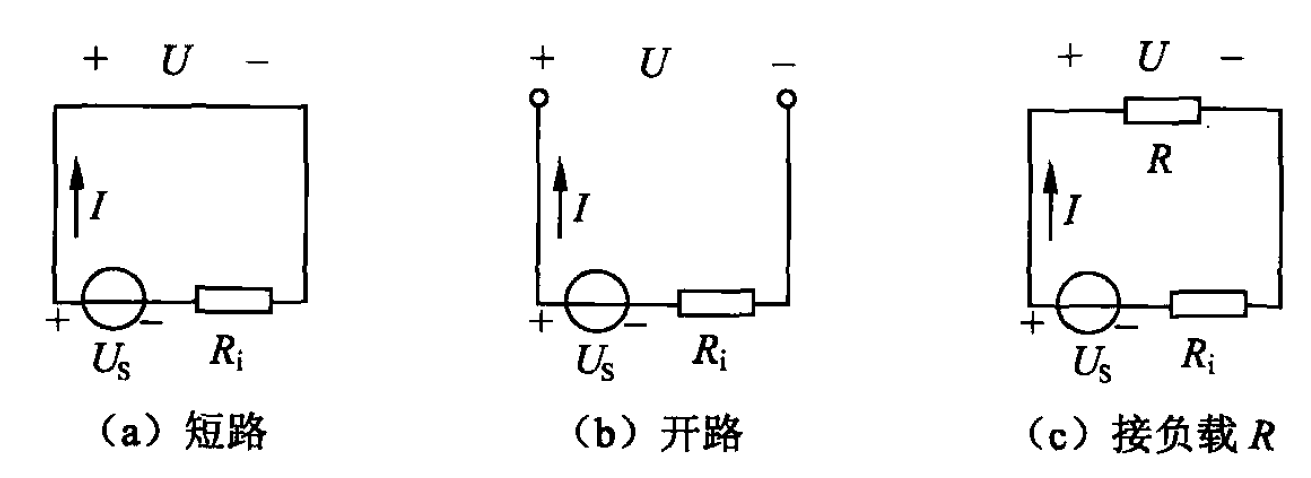
\includegraphics[width=0.6\textwidth]{assets/1/ae1cfc03fad5c98bfff08a663714a004.png}
\caption{\bfseries 1.1 习题集 1-2}
\end{figure}

\section{习题集 1-9: 求题图 (a) 中的电压 $U_{ab}$,图 (b) 中的电阻 $R$,图 (c) 中的电压 $U_S$ 和图 (d) 中的电流 $I$}

\begin{enumerate}
    \item[(a)]  $ \varphi_a - 3\ \mathrm{V} + 2\ \mathrm{V} = \varphi_b \Longrightarrow U_{ab} = 1\ \mathrm{V} $ 
    \item[(b)] $I = 1\ \mathrm{A},\  3 -IR= -4 \Longrightarrow R = 7\ \Omega$ 
    \item[(c)] $-3 + U_S = 1 \Longrightarrow U_S = 4 \ \mathrm{V}$ 
    \item[(d)] $R=2\ \Omega,\ -IR + 2 = 3 \Longrightarrow I = -0.5\ \mathrm{A}$ 
\end{enumerate}

\begin{figure}[H]\centering
    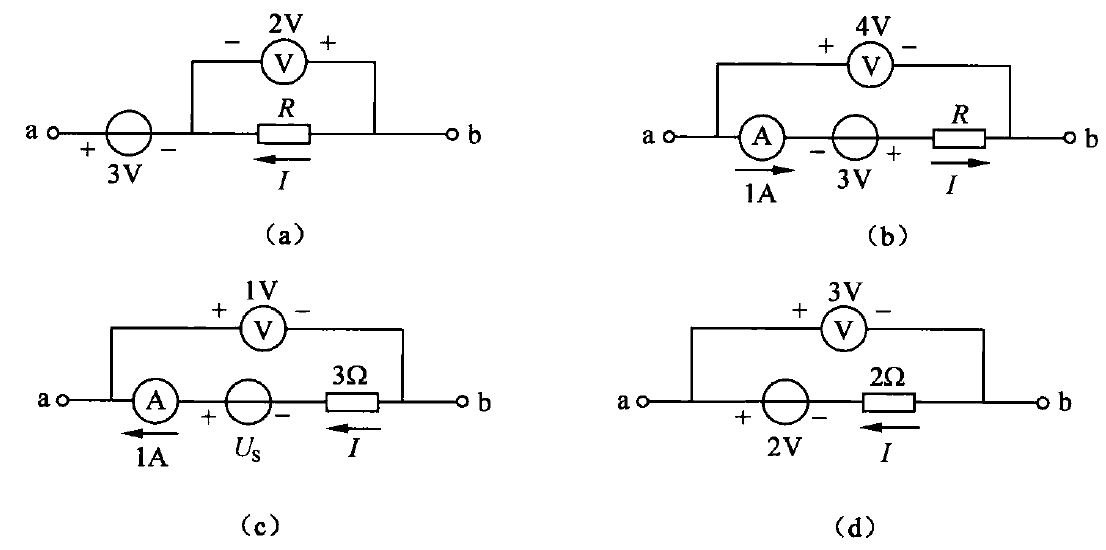
\includegraphics[width=0.6\textwidth]{assets/1/d3d69ecd6b1c1bc476fd4a4957fb9e56.png}
\caption{\bfseries 1.2 习题集 1-9}
\end{figure}

\section{习题集 1-10: 求题图电路中的电压 $U_{ab}$}



\begin{enumerate}
\item[(a)] 
记参考点 a 的电势 $\varphi_a=0$,则 $\varphi_c = 2\ \mathrm{V} ,\ \varphi_b = -2\ \mathrm{V}$,因此 $U_{ab} = 2\ \mathrm{V}$

\item[(b)] 
记参考点 d 的电势 $\varphi_d = \varphi_b =0$,则 $\varphi_c = 6\ \mathrm{V},\ \varphi_a = -2\ \mathrm{V}$,因此 $U_{ab} = -2\ \mathrm{V}$

\end{enumerate}

\begin{figure}[H]\centering
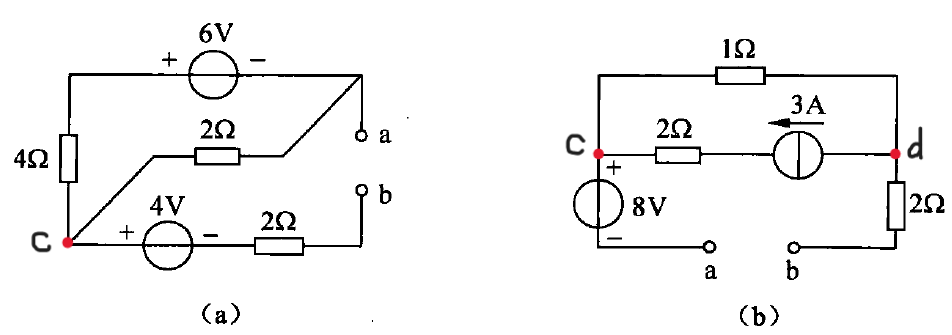
\includegraphics[width=0.55\textwidth]{assets/1/9dda9e5f333b8cb7f498d15c015e5fd0.png}
\caption{\bfseries 1.3 习题集 1-10}
\end{figure}
{\par\color{gray}\small
后补:(b) 中电流源两端仍有电势差,$\varphi_c \ne 6 \ \mathrm{V}$ 而是 $ \varphi_c = -3\ \mathrm{V} $,最终得 $U_{ab} = -5 \ \mathrm{V}$。
\par}


\section{习题集 1-15: 求题图各电路汇总所标出的电压和电流}

\begin{enumerate}
    \item[(a)] $I = -\frac{U}{R} + 4\ \mathrm{A} = -2 \ \mathrm{A}$
    \item[(b)] $U =12 \ \mathrm{V} + 3\ \Omega \times 4 \ \mathrm{A} = 0 $ 
    \item[(c)] $I = 8 \ \mathrm{A} - 6\ \mathrm{A} = 2 \ \mathrm{A}$,$ U = 12 \ \mathrm{V} + 3\times8 \ \mathrm{V} = 36 \ \mathrm{V}$ 
    \item[(d)] 取点 $ d $ 为参考点,则 $\varphi_d = \varphi_c = 0$,$\varphi_b = \varphi_a = 9 \ \mathrm{V}$,于是 $U_1 = 9 + 2\times3 = 15\ \mathrm{V},\ U_2 = 9 + 2\times 2 = 13 \ \mathrm{V},\ I =2 -  (9-3) = - 4 \ \mathrm{A}$
\end{enumerate}

\begin{figure}[H]\centering
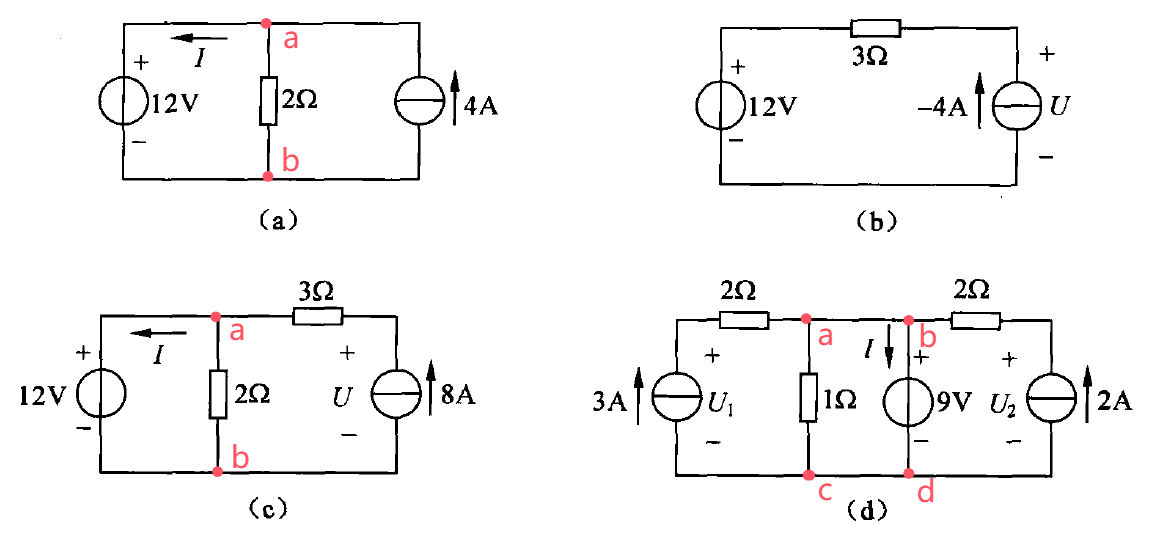
\includegraphics[width=0.7\textwidth]{assets/1/b82ef4f3b4efd9d0ee903e5f19353345.png}
\caption{\bfseries 1.4 习题集 1-15}
\end{figure}

\section{习题集 1-29: 题图电路中流过 $40\ \Omega$ 电阻的电流为 $2$ A,求电流源的电流值 $I_S$}

取点 $a$ 为参考点 $\varphi_a = 0$,可得 $\varphi_b = 100U_1 - 80$,于是在结点 $a$ 有电流:
\begin{equation*}
I_S + \frac{100U_1 - 80}{5} = 2
\end{equation*}

$0.2\ \Omega$ 电阻处又有 $U_1 = 0.2 I_S$,联立解得 $I_S = 3.6 \ \mathrm{A}, U_1 = 7.2 \ \mathrm{V}$。

\section{习题集 1-30: 求题图电路中独立电源的功率}

这里要注意左二元器件是受控电流源,因此 $0.5U$ 是指电流大小而非电压。$I_1$ 处可列出方程:

\begin{equation*}
\frac{U}{2} + 12 - \frac{U}{3} = 0.5U \Longrightarrow U = 36 \ \mathrm{V} \Longrightarrow P = UI = 432 \ \mathrm{W}
\end{equation*}

\begin{figure}[H]\centering
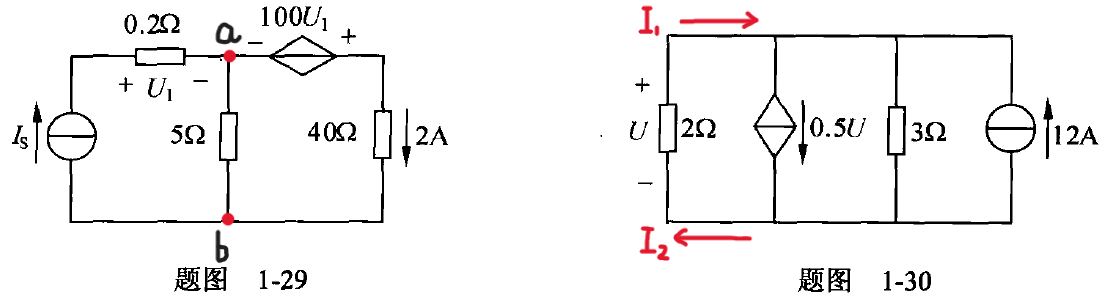
\includegraphics[width=0.7\textwidth]{assets/1/94b342032a5f6622a60b3c9d99e37993.png}
\caption{\bfseries 1.4 习题集 1-29 和 1.5 习题集 1-30}
\end{figure}

{\par\color{gray}\small
后补:上面的方程列错了,错将 $I_1$ 的方向标为由左向右,应该是由右向左。最后得到 $P = 108\ \mathrm{W}$。另外,也可以直接将受控电流源看作是 2 $\Omega$ 的电阻,这样左侧三个电阻并联,也可求出正确答案 108 W.
\par}


\section{讲义题 1-6: 关联参考方向下,电阻的 $\alpha > 90^\circ$ 代表什么物理意义}

$\alpha > 90 \text{\textdegree}$ 时,电阻为“负电阻”。

\section{讲义题 1-7: 充电电池的 1 C 是什么意思,涓流充电是多少 C,快速充电是多少 C}


\begin{definition}[充放电倍率 C 的含义]
C (充放电倍率)表示电池充放电时电流相对电池容量的大小数值,$\mathrm{C} = \frac{\text{电池容量}}{\text{充放电所需时间}}$。例如,1 C 电流充电表示电池需要 1 小时充满,5 C 充电表示电池需要 $0.2$ 小时充满。放电也是类似的,一个 10 Ah 的电池以 2 C 放电,表示以 20 A 的电流放电 0.5 h。 \par
若倍率上升,总时间就会下降,若倍率下降,总时间就会上升。通俗来讲,$C$ 代表了电池的爆发力大小,高倍率的动力电池瞬间放电电流大,特别适合大电流放电产品使用,如航模。
\end{definition}


\begin{definition}[涓流充电]
涓流充电是指在电池接近完全充满电后,采用非常小的电流进行充电,以弥补电池自放电造成的容量损失。理论倍率 C 约为 最大倍率 $\mathrm{C_{max}}$ 的 $\frac{1}{100}$ 至 $\frac{1}{1000}$,但由于倍率太小,常常根本无法充电,一个比较好的方法是脉冲式充电,例如以 $\frac{\mathrm{C_{max}}}{10}$ 充电 6 s,然后停止充电 54 s。
\end{definition}


\begin{definition}[快速充电]
快速充电至少要求 1 C,现阶段的快速充电多在 1.5 C 至 2 C 之间。
\end{definition}


\section{讲义题 1-8(Multisim 仿真): 用 Multisim 实现课堂仿真中的 MOSFET。画出 $U_{GS}$ 固定为 5 V,$U_{DS}$(横轴)从 0 V 到 12 V 变化时 $I_{DS}$(纵轴)的曲线;以及 $U_{DS}$ 固定为 10 V,$U_{GS}$(横轴)从 0 至 10 V 变化时 $I_{DS}$(纵轴)的曲线}

仿真电路如图 \ref{仿真电路图} 所示,

\begin{figure}[H]\centering
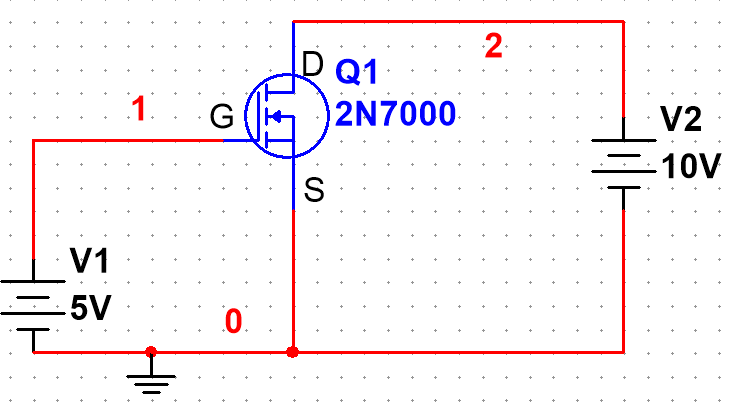
\includegraphics[width=0.36\textwidth]{assets/1/5c45ed5b5258df3fa8e1babac4a7ace2.png}
\caption{\textbf{仿真电路图}}\label{仿真电路图}
\end{figure}

先固定 $U_{GS} = 5\ \mathrm{V}$ 不变(即 $V_1 = 5\ \mathrm{V}$),横坐标 $U_{DS} \in [0\ \mathrm{V},\ 12\ \mathrm{V}]$,画出 $I_{DS}$(即 $I_2$)的变化曲线,如图 \ref{仿真结果1} 所示。再固定 $U_{DS} = 10\ \mathrm{V}$ 不变(即 $V_2 = 10\ \mathrm{V}$),横坐标 $U_{GS} \in [0\ \mathrm{V},\ 10\ \mathrm{V}]$,画出 $I_{DS}$(即 $I_2$)的变化曲线,如图 \ref{仿真结果2} 所示。
\begin{center}
    \noindent\begin{minipage}{0.42\textwidth}
        \begin{figure}[H]\centering
        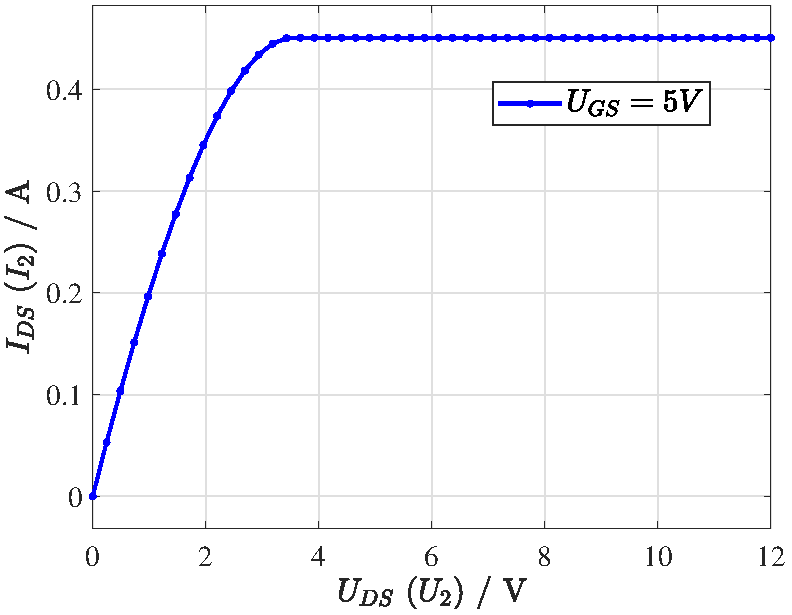
\includegraphics[width=\textwidth]{assets/1/2024-08-30_00-57-32.pdf}
        \caption{\textbf{仿真结果1}}\label{仿真结果1}
        \end{figure}
    \end{minipage}\hspace{5mm}
    \begin{minipage}{0.42\textwidth}
        \begin{figure}[H]\centering
        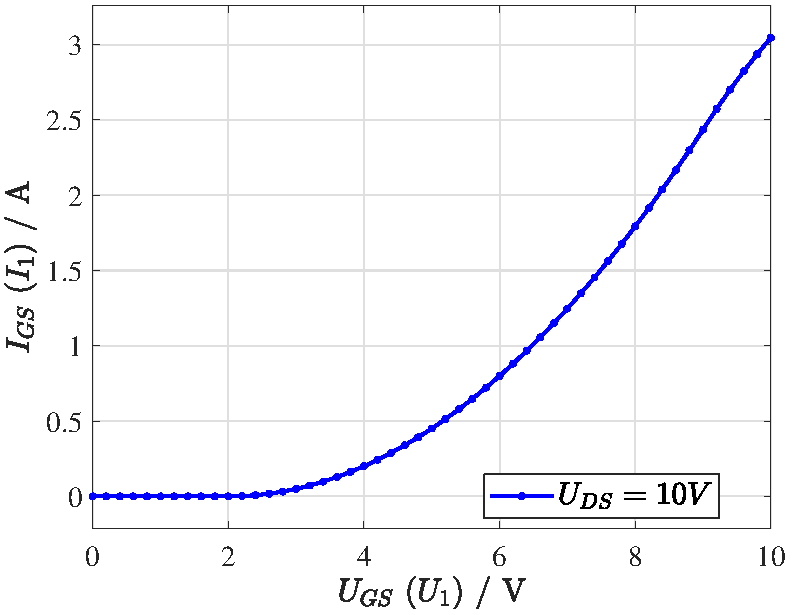
\includegraphics[width=\textwidth]{assets/1/2024-08-30_00-57-34.pdf}
    \caption{\textbf{仿真结果2}}\label{仿真结果2}
    \end{figure}
    \end{minipage}
\end{center}



\chapter{Homework 2: 2024.9.3 - 2024.9.9}\thispagestyle{fancy}

\section{习题集 1-33: 题图电路中 $R_1 = 40$,$R_e = 27$,$R_b = 150$,$R_L = 1500$,单位都为 $\Omega$,$\alpha = 0.98$,求电压增益 $\frac{u_2}{u_1}$ 和功率增益 $\frac{p_2}{p_1}$,其中 $p_1$ 是 $u_1$ 输出的功率,$p_2$ 是 $R_L$ 吸收的功率}
左半边回路有:
\begin{gather*}
u_1 - 67i_e - (1-\alpha)i_e \cdot 150 = 0 \Longrightarrow \frac{u_2}{u_1} = \frac{\alpha i_eR_L }{70i_e} = \frac{0.98\times 1500}{70} = 21 \\ 
p_2 = (\alpha i_e)^2R_L, \quad p_1 = u_1 i_e \Longrightarrow \frac{p_2}{p_1} = \frac{(\alpha i_e)^2R_L}{70i_e^2} = 20.58
\end{gather*}

\begin{figure}[H]\centering
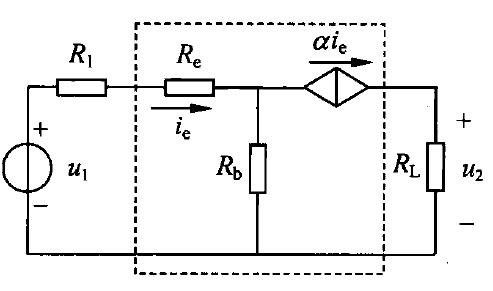
\includegraphics[width=0.5\textwidth]{assets/2/image (47).jpg}
\caption{\textbf{习题集 1-33}}
\end{figure}


\section{习题集 2-2: 求题图各电路的入端电阻 $R$}
对图 (a),化简并联后电桥平衡,可以得到
\begin{equation*}
\frac{1}{R} = \frac{1}{20 } + \frac{1}{40} +\frac{1}{40} \Longrightarrow R = 10\ \Omega
\end{equation*}
对图 (b),经过多次并联化简,可以得到:
\begin{equation}
R = 8 + \frac{3\times 6}{3+6}=10\ \Omega
\end{equation}
\begin{figure}[H]\centering
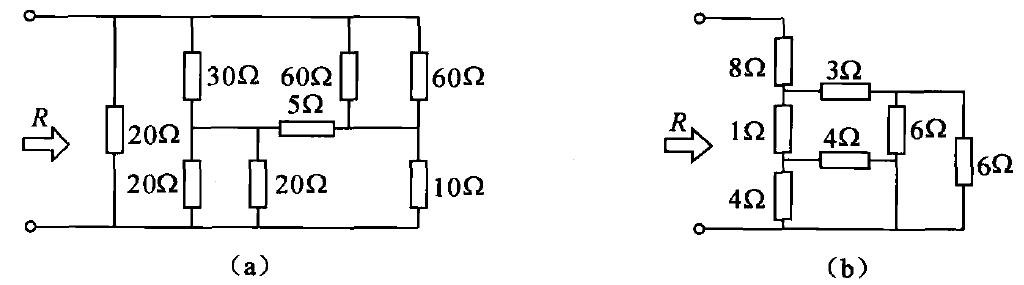
\includegraphics[width=0.85\textwidth]{assets/2/e02c39d3f229a4b6352b828e57c3737f.jpg}
\caption{\textbf{习题集 2-2}}
\end{figure}

\section{习题集 2-6: 将题图中各电路化为最简电路}

各电路的最简电路图如图 \ref{习题集 2-6 解答} 所示: 

\noindent\begin{minipage}{0.50\textwidth}
    \begin{figure}[H]\centering
        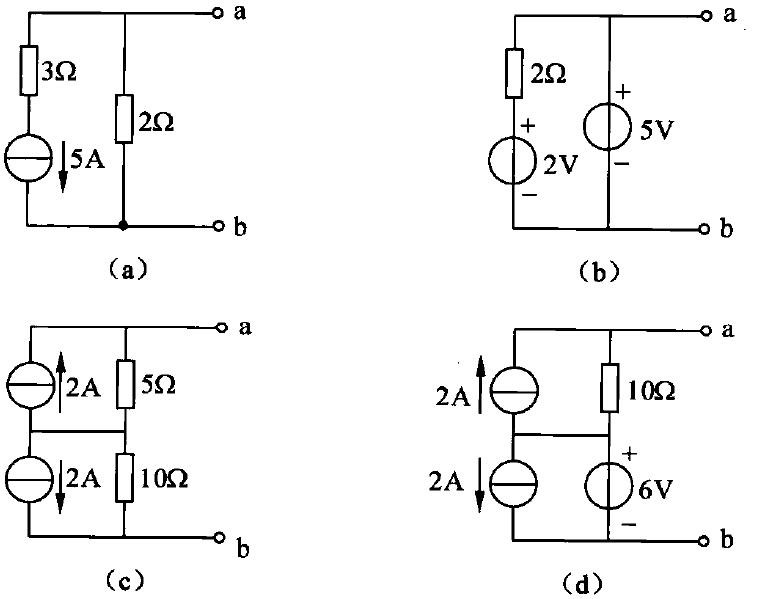
\includegraphics[height=185pt]{assets/2/bfc7d58924b9eaf9582656c984bd2c3b.jpg}
        \caption{\textbf{习题集 2-6}}
    \end{figure}
\end{minipage}\hfill
\begin{minipage}{0.50\textwidth}
    \begin{figure}[H]\centering
        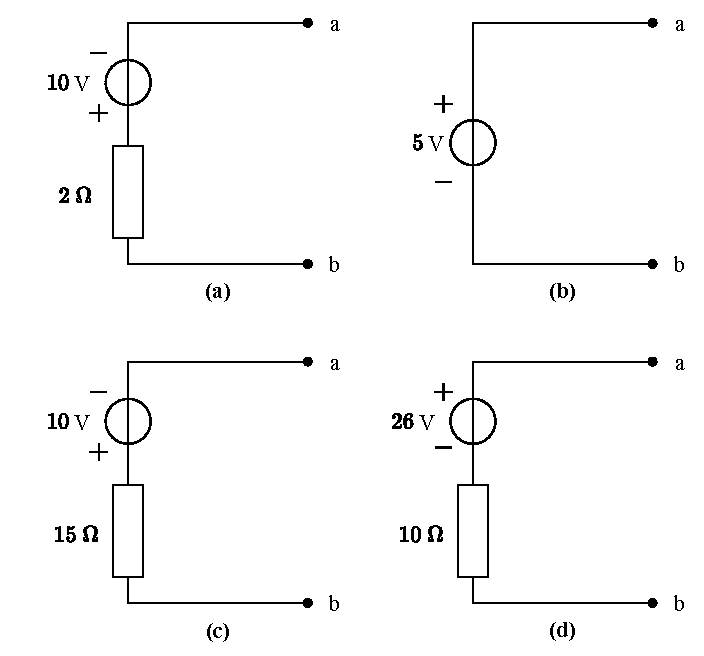
\includegraphics[height=185pt]{assets/2/2-6.drawio.pdf}
        \caption{\textbf{习题集 2-6 解答}}\label{习题集 2-6 解答}
    \end{figure}        
\end{minipage}


\section{习题集 2-8: 用电源等效方法求题图中的电流 $i$}

对原电路进行多次等效转换,得到最简电路如图所示,进而有:
\begin{equation*}
I = \frac{3}{2+3+5} = 0.3\ \mathrm{A}
\end{equation*}

\noindent\begin{minipage}{0.49\textwidth}
    \begin{figure}[H]\centering
        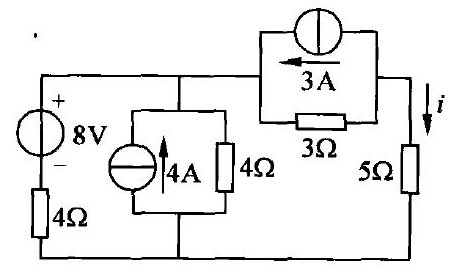
\includegraphics[height=110pt]{assets/2/78abd22edee32bbd38134d510246a9ab.jpg}
        \caption{\textbf{习题集 2-8}}
    \end{figure}
\end{minipage}\hfill
\begin{minipage}{0.49\textwidth}
\begin{figure}[H]\centering
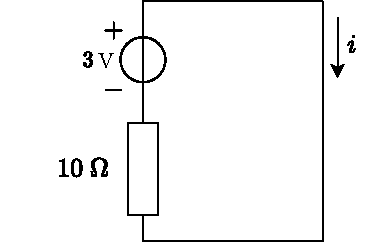
\includegraphics[height=110pt]{assets/2/2-8.drawio.pdf}
\caption{\textbf{习题集 2-8 等效电路}}\label{习题集 2-8 等效电路}
\end{figure}
\end{minipage}

\section{习题集 2-11: 求题图中的电流 $I$}

等效电路图如图 \ref{习题集 2-11 等效电路} 所示,由 KVL 得:
\begin{gather*}
28 = 4I' + 4(I' - I),\quad 25 = -8I + 4(I' - I) \Longrightarrow I' = 2.95\ \mathrm{A},\ I = -1.1\ \mathrm{A}
\end{gather*}


\noindent\begin{minipage}{0.55\textwidth}
\begin{figure}[H]\centering
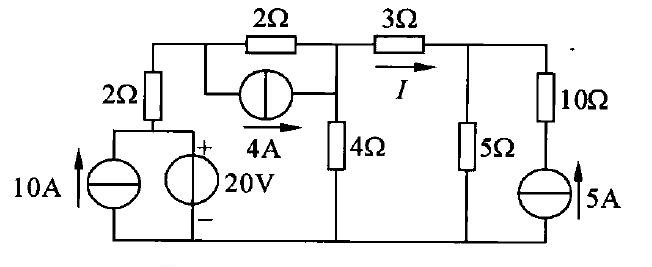
\includegraphics[height=105pt]{assets/2/1187c3e12fa1e6bd8d2019d53bd2752a.jpg}
\caption{\textbf{习题集 2-11}}
\end{figure}
\end{minipage}\hfill
\begin{minipage}{0.43\textwidth}
\begin{figure}[H]\centering
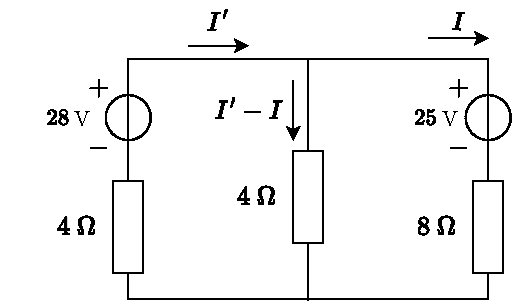
\includegraphics[height=105pt]{assets/2/2-11.drawio.pdf}
\caption{\textbf{习题集 2-11 等效电路}}\label{习题集 2-11 等效电路}
\end{figure}
\end{minipage}

\section{习题集 2-17: 求题图中的电压 $U_{ab}$}

等效电路图如图 \ref{2-17} 所示,可以求得:
\begin{equation*}
4I - 8 = 12(I-1) \Longrightarrow I = 0.5\ \mathrm{A}\Longrightarrow U_{ab} = 8 - 8I = 4\ \mathrm{V}
\end{equation*}


\noindent\begin{minipage}{0.49\textwidth}
\begin{figure}[H]\centering
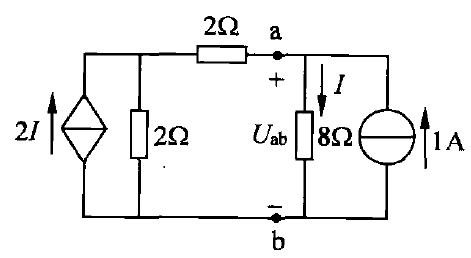
\includegraphics[height=120pt]{assets/2/78473b1c403974e048249bbdbf6a152f.jpg}
\caption{\textbf{习题集 2-17}}
\end{figure}
\end{minipage}\hfill
\begin{minipage}{0.49\textwidth}
\begin{figure}[H]\centering
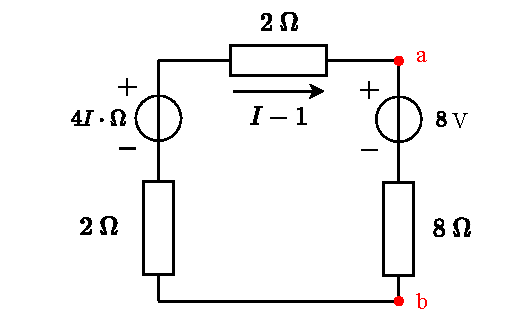
\includegraphics[height=120pt]{assets/2/2-17.drawio.pdf}
\caption{\textbf{习题集 2-17 等效电路}}\label{2-17}
\end{figure}
\end{minipage}



\section{习题集 2-22: 求题图中的电压 $U_1$,$U_2$ 和电流源发出的功率}

经过电源等效和 $\Delta$-Y 变换,等效电路图如图 \ref{2-22} 所示,回路总电阻 $R = 3 + \frac{4}{9} + \frac{14}{9} = 5\ \Omega$,\ $I_1 = \frac{U}{R} = 1.2\ \mathrm{A}$,则有:
\begin{equation*}
U_1 = 6 - 3\times 1.2 = 2.4\ \mathrm{V},\ U_2 = 2\times \frac{I}{2} = 1.2\ \mathrm{V},\quad P = 2 U_1 = 4.8\ \mathrm{W}
\end{equation*}

\noindent\begin{minipage}{0.49\textwidth}
\begin{figure}[H]\centering
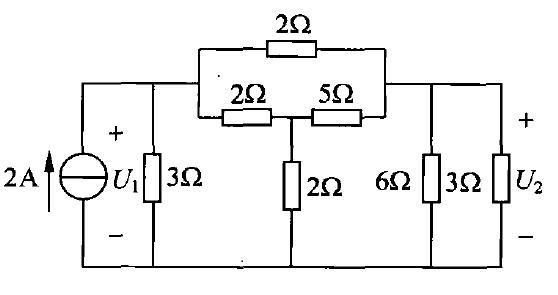
\includegraphics[height=110pt]{assets/2/0c8d1f0fb90ef6983c0aef6451919e4b.jpg}
\caption{\textbf{习题集 2-22}}
\end{figure}
\end{minipage}\hfill
\begin{minipage}{0.49\textwidth}
\begin{figure}[H]\centering
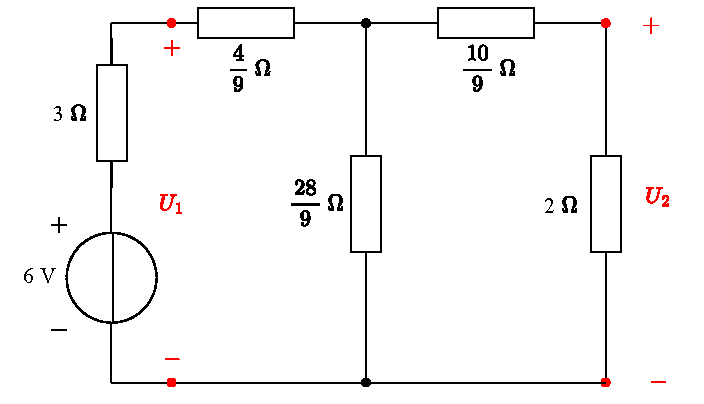
\includegraphics[height=110pt]{assets/2/2-22.drawio.pdf}
\caption{\textbf{习题集 2-22}}\label{2-22}
\end{figure}
\end{minipage}

%\newpage
%\section{\color[rgb]{0.2,0.9,0.2}(非作业) 习题集 2-4 (b)}
%\section{\color[rgb]{0.2,0.9,0.2}(非作业) 习题集 2-5}
%\section{\color[rgb]{0.2,0.9,0.2}(非作业) 习题集 2-5}



\chapter{Homework 3: 2024.9.10 - 2024.9.18}\thispagestyle{fancy}


\section{习题集 3-40(书上答案不正确): 题图电路中,$u_s(t) = \sin 4t\ \mathrm{V} $,电阻 $R_2 = 2R_1 = 1 \kO$,求电流 $i(t)$}

由虚短和虚断,可以得到 $R_1$ 处电流为 $i_1 = \frac{u_s}{R_1}$(从上至下),于是输出电压 $u_o = 3u_s$,右侧负载由三个电阻构成,并联电阻分压 $2u_s$,最后得电流 $i(t)$:
\begin{equation}
i(t) = \frac{2u_s}{6 \KO} = \frac{u_s}{3} \mA
\end{equation}

\begin{figure}[H]\centering
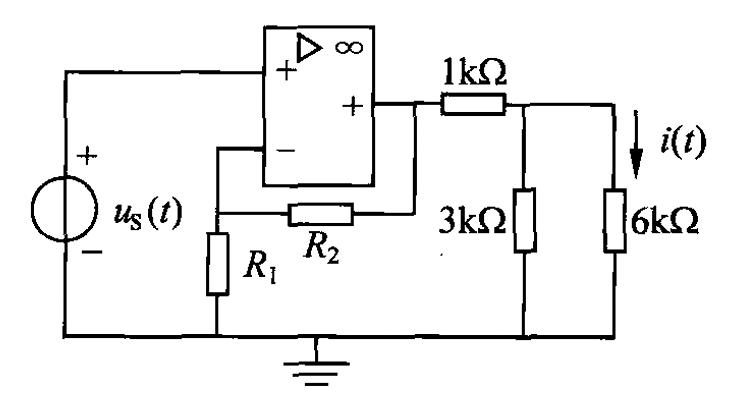
\includegraphics[width=0.35\textwidth]{assets/3/3-40.jpg}
\caption{\bfseries 习题集 3-40}
\end{figure}

\section{习题集 3-45(注意题目单位是 S): 对题图电路,求电压增益 $\frac{U_o}{U_i}$ 和入端电阻 $R_i$}

如图所示,将电导全部转换为电阻。由虚断、虚短,流经 $\frac{1}{10}\ \Omega$ 电阻的电流为 $i_1 = \frac{u_s}{0.1\ \Omega} = 10u_s$。右下角两电阻分压,再由虚短可得 $i_2 = 2U_o$,于是 $i_3 = i_1 + i_2 = 10 U_s + 2U_o$,由 KVL:
\begin{equation}
0 - \frac{1}{3}(10 U_s + 2U_o) = U_o \Longrightarrow  \frac{U_o}{U_s} = -2
\end{equation}
入端电阻 $R_i$: 
\begin{equation}
    i_1 = 10U_s \Longrightarrow  R_i = \frac{1}{10}\ \Omega
\end{equation}

\section{习题集 3-46: 题图电路中,$R_1 = R_2 = R_3 = R_4 = R_o = R_L$,求在输入电压 $u_i$ 作用下的负载电流 $i_L$}

依据 KVL、KCL、虚短、虚断,标出各节点电势,如图所示。则有:
\begin{equation}
(u_i+u_o)-u_o = i_LR,\ i_L = \frac{u_o}{R_L} \Longrightarrow u_o = u_i,\ i_L = \frac{u_o}{R_L} = \frac{u_i}{R_L}
\end{equation}

\begin{figure}[H]\centering
    \begin{subfigure}[t]{0.43\textwidth}\centering
        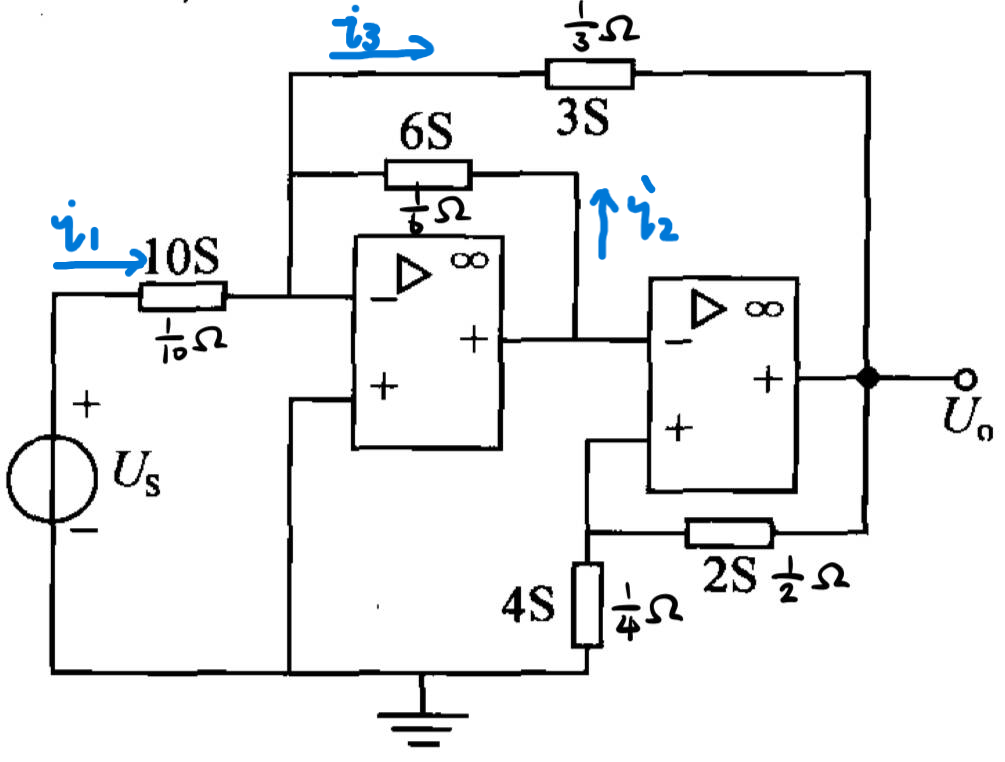
\includegraphics[height=130pt]{assets/3/3-45.png}
        \caption{\bfseries 习题集 3-45 }
    \end{subfigure}\begin{subfigure}[t]{0.43\textwidth}\centering
        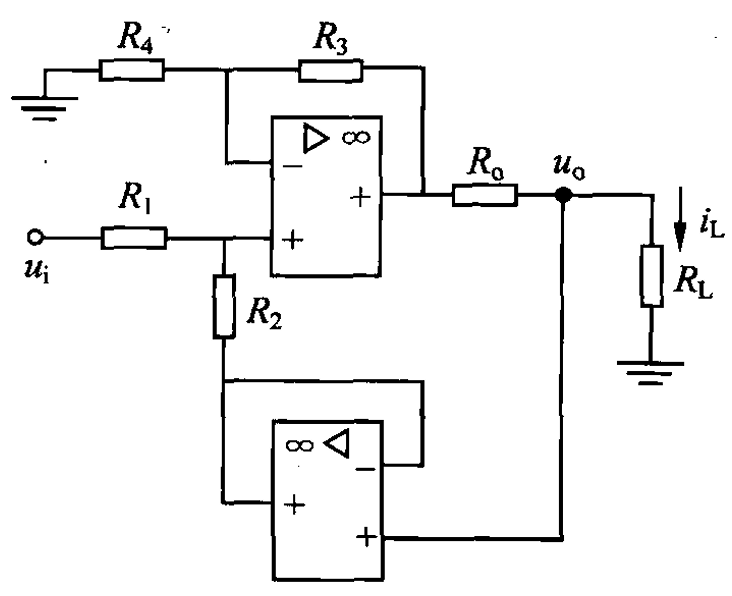
\includegraphics[height=130pt]{assets/3/3-46.png}
        \caption{\bfseries 习题集 3-46 }
    \end{subfigure}
    \caption{\bfseries 习题集 3-45 和习题集 3-46 }
    \end{figure}
    


\section{讲义题 2-19: 求同相比例放大器和反向比例放大器的输入电阻和输出电阻,放大器均理想,根据求解结果讨论两种放大器的优劣}
\textbf{(1)\ 反相比例放大器}

对输入电阻,$i_1 = \frac{u_i}{R_1} \Longrightarrow R_i = R_1$。对输出电阻,将输入电压源短路,采用加流求压法,在输出端接入电流源,由 $u = iR$ 且 $u=0$,得 $R_o = 0$。也即:
\begin{equation}
R_i = R_1,\ R_o = 0
\end{equation}

\textbf{(2)\ 同相比例放大器}

对输入电阻,$R_1$ 右端断路,因此 $R_i = \infty$。对输出电阻,将输入电压源短路,采用加流求压法,在输出端接入电流源,由 $u = iR$ 且 $u=0$,得 $R_o = 0$。也即:
\begin{equation}
R_i = \infty,\ R_o = 0
\end{equation}

从输入输出电阻特性来看,同相比例放大器电气特性更优秀。

\begin{figure}[H]\centering
\begin{subfigure}[t]{0.4\textwidth}\centering
    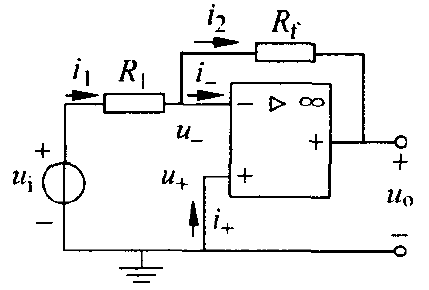
\includegraphics[height=100pt]{assets/3/反向比例放大器.png}
    \caption{\bfseries 同相比例放大器}
\end{subfigure}\begin{subfigure}[t]{0.4\textwidth}\centering
    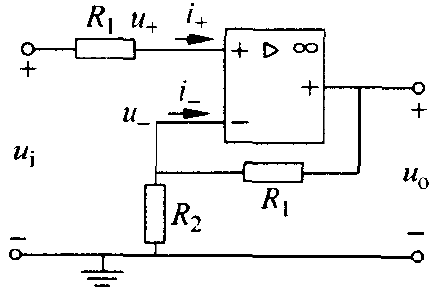
\includegraphics[height=100pt]{assets/3/同相比例放大器.png}
    \caption{\bfseries 反向比例放大器}
\end{subfigure}
\caption{\bfseries 讲义题 2-19}
\end{figure}

\section{讲义题 2-20: 求题图各网络的 $\boldsymbol{G}$ 参数}
\textbf{(a)} 由 KVL 有:
\begin{equation}
\begin{cases}
    u_1 = R_2(i_1 - i_2) \\
    u_2 = R_1 i_2 
\end{cases}\Longrightarrow  
\begin{cases}
    i_1 = \frac{1}{R_2}u_1 + \frac{1}{R_1}u_2 \\ 
    i_2 = \frac{1}{R_1}u_2 
\end{cases},\ 
\boldsymbol{G} = 
\begin{bmatrix}
    \frac{1}{R_2} & \frac{1}{R_1} \\ 
    \frac{1}{R_1} & 0
\end{bmatrix}
\end{equation}

\textbf{(b)} 由 KVL, KCL 有:
\begin{equation}
\begin{cases}
    u_1 = R_1\left( i_1 - \frac{u_1 - u_2}{R_2} \right)\\
    u_2 = R_1 \left( i_2 + \frac{u_1 - u_2}{R_2} \right)
\end{cases}\Longrightarrow  
\begin{cases}
    i_1 = \left( \frac{1}{R_1} + \frac{1}{R_2} \right)u_1 - \frac{1}{R_2}u_2 \\ 
    i_2 =  - \frac{1}{R_2}u_1  + \left( \frac{1}{R_1} + \frac{1}{R_2} \right)u_2\\ 
\end{cases},\ 
\boldsymbol{G} = 
\begin{bmatrix}
    \frac{1}{R_1} + \frac{1}{R_2} & -\frac{1}{R_2} \\ 
    -\frac{1}{R_2} & \frac{1}{R_1} + \frac{1}{R_2}
\end{bmatrix}
\end{equation}

\begin{figure}[H]\centering
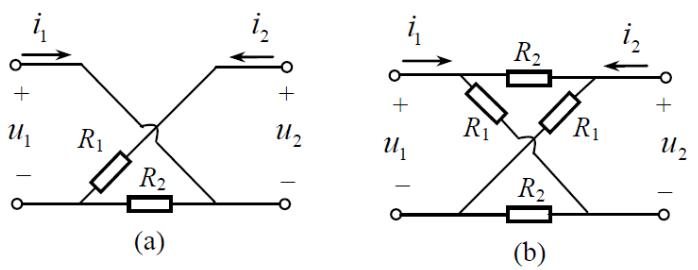
\includegraphics[width=0.55\textwidth]{assets/3/image (8).jpg}
\caption{\bfseries 讲义题 2-20}\label{讲义题 2-20}
\end{figure}


\chapter{Homework 4: 2024.9.19 - 2024.9.24}\thispagestyle{fancy}

\section{讲义题 2-20: 求图示各网络的 和 $\boldsymbol{R}$ 参数}


如图 \ref{求G参数} (a),对 (a) 电路有:
\begin{equation}
\begin{cases}
    u_1 + u_2 = i_2R_1 \\ 
    u_1 = (i_1 - i_2)R_2 \\ 
\end{cases}
\Longrightarrow 
\begin{cases}
    u_1 = R_2 i_1 + (-R_2)i_2 \\ 
    u_2 = (-R_1)i_1 + (R_1+R_2)i_2
\end{cases},\ 
\boldsymbol{R} = 
\begin{bmatrix}
    R_2 & -R_2 \\ 
    -R_1 & R_1+R_2
\end{bmatrix}
\end{equation}

对 (b) 电路,设 2 号端口的低电位为 $u$,也即 $u_{2,-} = u$,由 KCL: 
\begin{gather}
\begin{cases}
    i_1 + \frac{u+u_2 - u_1}{R_2} = \frac{u_1 - u}{R_1} \\ 
    \frac{u_1 - u}{R_1} = i_2 + \frac{u}{R_2} \\ 
    \frac{u+u_2}{R_1} + \frac{u}{R_2} = i_1
\end{cases}
\Longrightarrow
\begin{cases}
    u_1 + u_2 = R_1i_1 + R_1i_2 \\ 
    u_1 - u_2 = R_2i_1 - R_2i_2
\end{cases} 
\\
\Longrightarrow 
\begin{cases}
    u_1 = \frac{R_1+R_2}{2}i_1 + \frac{R_1-R_2}{2}i_2 \\
    u_2 = \frac{R_1-R_2}{2}i_1 + \frac{R_1+R_2}{2}i_2
\end{cases},\ 
\boldsymbol{R} = 
\begin{bmatrix}
    \frac{R_1+R_2}{2} & \frac{R_1-R_2}{2} \\ 
    \frac{R_1-R_2}{2} & \frac{R_1+R_2}{2}
\end{bmatrix}
\end{gather}



\section{讲义题 2-21: 图示电路中 $R_1 = 10\ \Omega$,$R_2 = 40\ \Omega$,求}

\noindent \textbf{(1)\ \ 此二端口网络的 $\boldsymbol{T}$ 参数:}

$i_1 = \frac{u_2}{R_2} + (-i_2),\quad u_1 = u_2 - R_1(i_2 - \frac{u_2}{R_2})$,得到此二端口的 $\boldsymbol{T}$ 参数:
\begin{equation}
\boldsymbol{T} = 
\begin{bmatrix}
    1 + \frac{R_1}{R_2} & R_1 \\ 
    \frac{1}{R_2} & 1
\end{bmatrix}
=
\begin{bmatrix}
    \frac{5}{4} & 10\  \Omega \\ 
    \frac{1}{40} \ \mathrm{S} & 1
\end{bmatrix}
\end{equation}

\noindent \textbf{(1)\ \ 求 $U_{S1}$ 和 $I_1$}

$(-i_2) = I_2 = 2\ \mathrm{A},\quad u_2 = I_2R_3 = 40\ \mathrm{V}$,代入即得:
\begin{equation}
\begin{bmatrix}
    U_{S1} \\ 
    I_1
\end{bmatrix}
= 
\boldsymbol{T}\cdot 
\begin{bmatrix}
    40\ \mathrm{V} \\ 
    2 \ \mathrm{A}
\end{bmatrix}
= 
\begin{bmatrix}
    70\ \mathrm{V} \\ 
    3 \ \mathrm{A}
\end{bmatrix}
\end{equation}

\begin{figure}[H]\centering
\begin{subfigure}[t]{0.4\columnwidth}\centering
    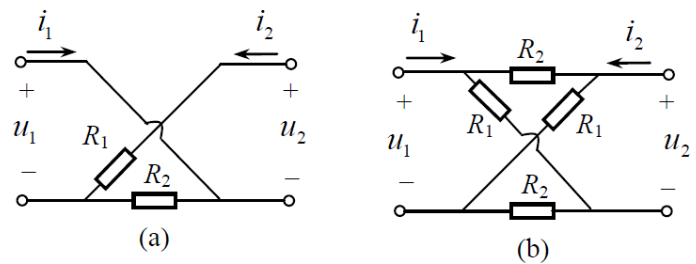
\includegraphics[height=76pt]{assets/4/ffe92b96174b737b0ba9725eef3dd53e.png}
    \caption{\bfseries 讲义题 2-20 图 }
\end{subfigure}\begin{subfigure}[t]{0.6\columnwidth}\centering
    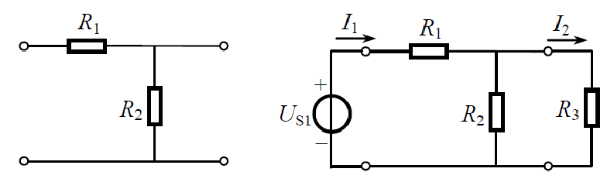
\includegraphics[height=76pt]{assets/4/a3822dcee8e6253ad95a943b6b83e06e.png}
    \caption{\bfseries 讲义题 2-21 图 }
\end{subfigure}
\caption{\bfseries 讲义题 2-20、讲义题 2-21 }\label{求G参数}
\end{figure}

\section{讲义题 2-22: 图示电路中二端口网络的 $\boldsymbol{T}$ 参数为 $\boldsymbol{T} = \begin{bmatrix} 2 & 8\  \Omega \\ 0.5\ \mathrm{S} & 2.5 \end{bmatrix} $}

\noindent \textbf{(1)\ \ 求此二端口的等效电路}

$\boldsymbol{T}$ 参数满足 $\det \boldsymbol{T} = 5 - 4 = 1$,也即满足互易条件,因此可以等效为 T 型三电阻电路,如图 \ref{} 所示。此时的电阻阻值为:
\begin{equation}
R_T = \frac{1}{T_{21}} = 2 \ \Omega,\quad R_a = R_T(T_{11} - 1) = 2\ \Omega,\quad R_b = R_T(T_{22} - 1) = 3\ \Omega
\end{equation}

\noindent \textbf{(1)\ \ $R_2$ 为何值时其获得最大功率}

$R_2$ 吸收的功率为 $p = \frac{u_2^2}{R_2}$,回路总电阻为 $2 + 2 + 2 \parallel (3 + R_2) = 4 + \frac{2(3+R_2)}{5+R_2}$,由分压原理得到 $u_2$:
\begin{equation}
u_2 = 6\cdot \frac{\frac{2(3+R_2)}{5+R_2}}{4 + \frac{2(3+R_2)}{5+R_2}} \cdot \frac{R_2}{ 3 + R_2} = \frac{6}{3+\frac{13}{R_2}}
\end{equation}
于是 $R_2$ 上的功率 $p$ 为:
\begin{equation}
p = \frac{u_2^2}{R_2} = \frac{36}{\frac{13^2}{R_2} + 78 + 9R_2} \leqslant \frac{36}{2\cdot 13 \cdot 3 + 78} \ \mathrm{W} = \frac{9}{39}\ \mathrm{W} = 0.2308 \ \mathrm{W}
\end{equation}
当且仅当 $\frac{13^2}{R_2} = 9R_2$ 取等,此时 $R_2 = \frac{13}{3}\ \Omega$。

事实上,视 $R_2$ 为负载,视电路的剩余部分为电源,可求得电源的内阻(也即输出电阻)为 $R_s = \frac{13}{3}\ \Omega$,因此当 $R_2 = R_s =  \frac{13}{3}\ \Omega$ 时,外部电路(也即负载 $R_2$)有最大功率。 

\begin{figure}[H]\centering
\begin{subfigure}[t]{0.4\columnwidth}\centering
    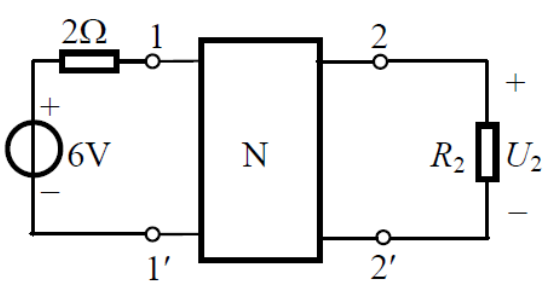
\includegraphics[height=110pt]{assets/4/199279d29390a5449f7ef5c5dc7f8a3d.png}
    \caption{\bfseries 讲义题 2-22 图 }
\end{subfigure}\begin{subfigure}[t]{0.6\columnwidth}\centering
    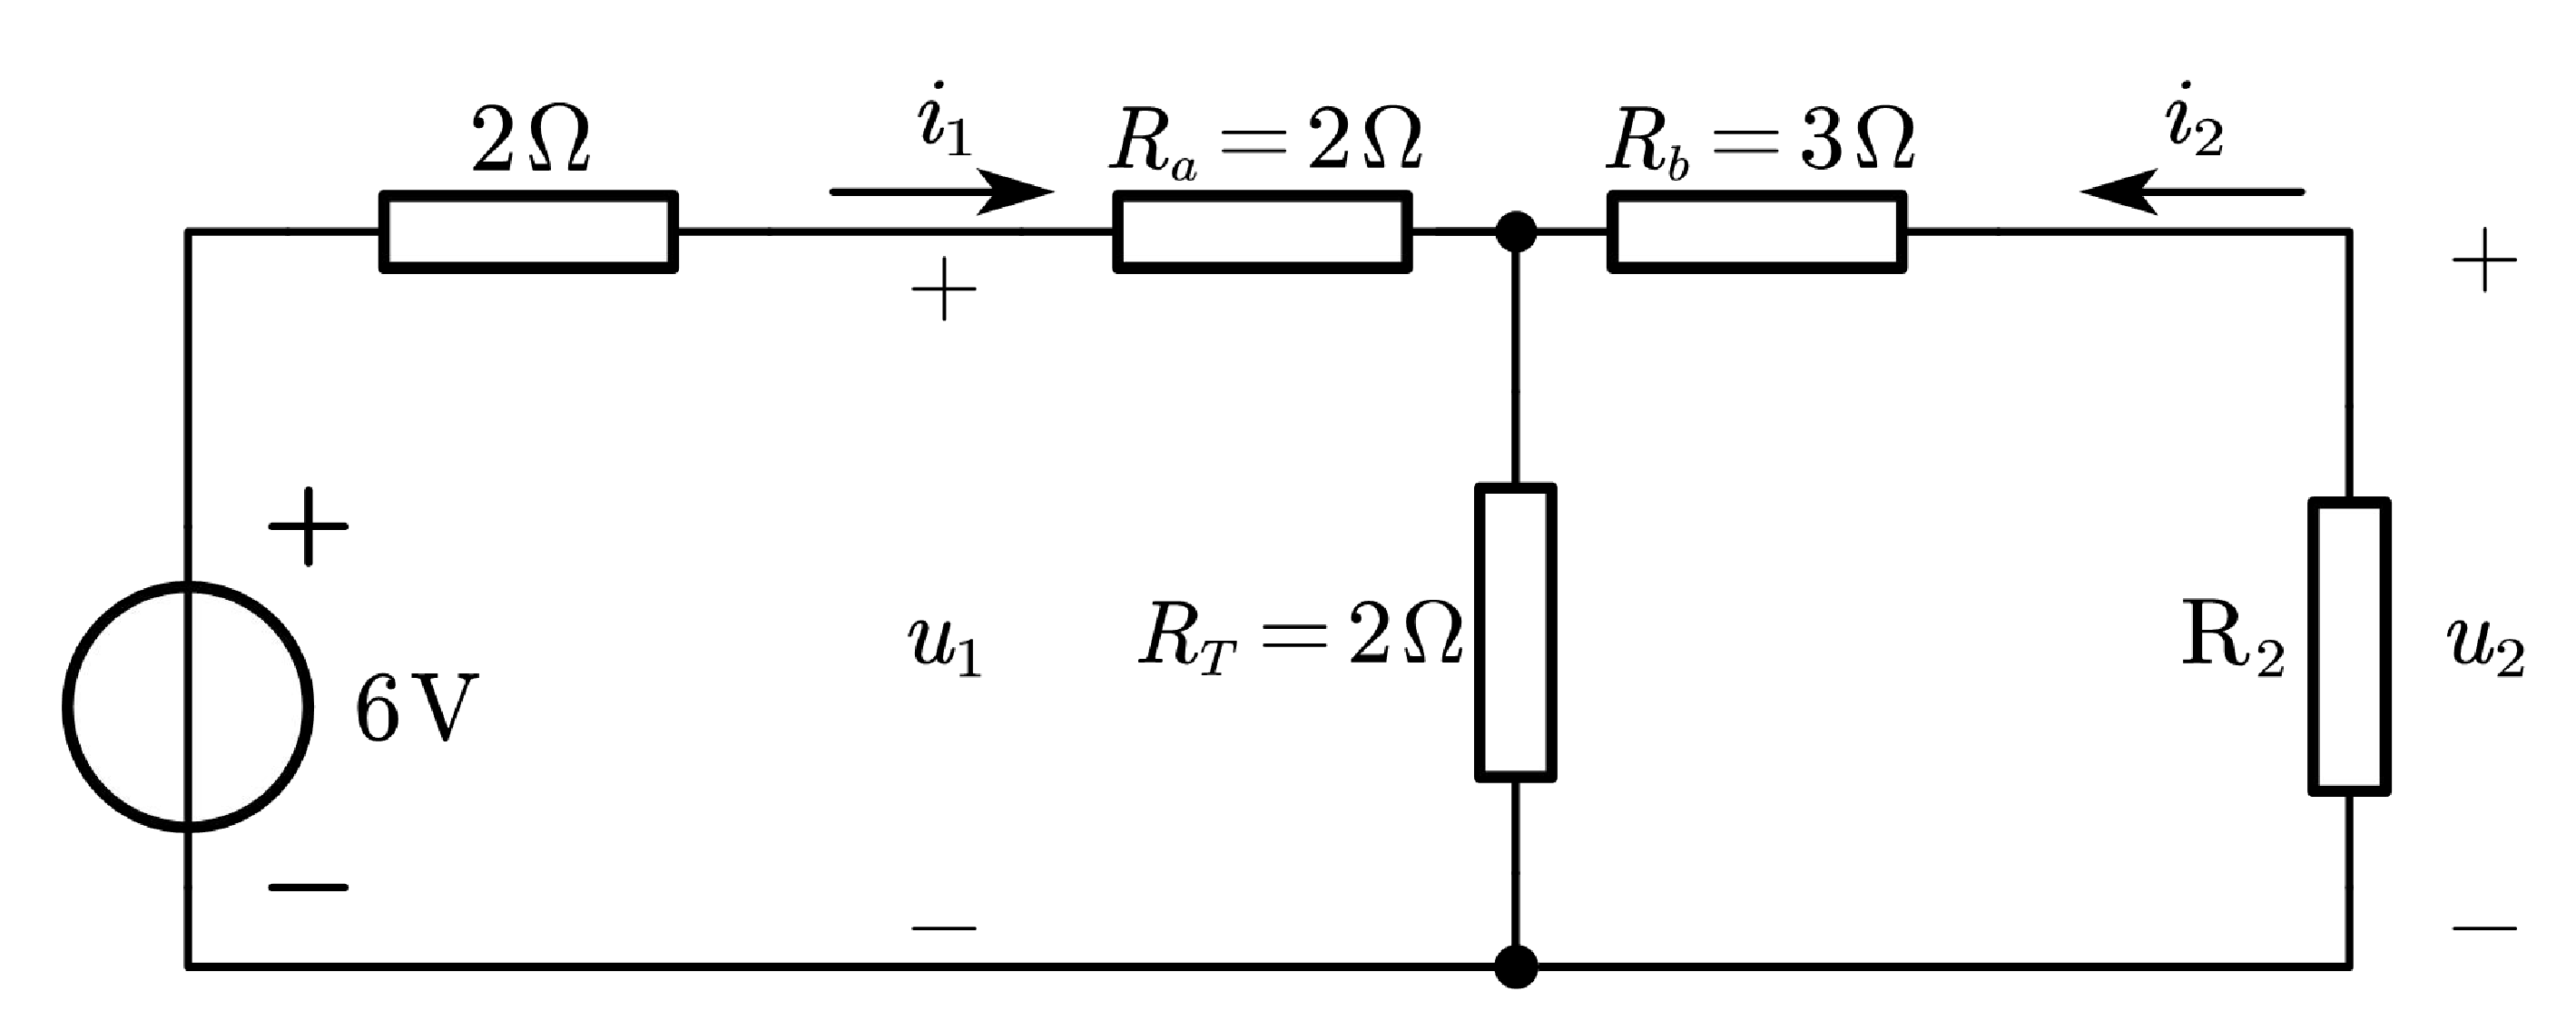
\includegraphics[height=110pt]{assets/4/2-22.pdf}
    \caption{\bfseries 讲义题 2-20 等效电路 }
\end{subfigure}
\caption{\bfseries 讲义题 2-22 }
\end{figure}


\chapter{Homework 5: 2024.9.25 - 2024.10.8}\thispagestyle{fancy}

\section{教材 2-41: 求由 N-E MOS 构成的两输入 NAND 和两输入 NOR 的最大功率,并指出何时有最大功率}

对于 NAND,仅当两输入都为 1 时有静态功率,也即最大功率,设 N-E MOS 的导通电阻为 $R_{\text{ON}}$,外接电阻 $R_L$,电源电压 $U_S$,则功率为:
\begin{equation}
    P_{\,\text{NAND, max}} = \frac{U_S^2}{R_L + 2R_{\text{ON}}}
\end{equation}

对于 NOR,任一输入为 1 时都具有静态功率,两输入都为 1 时有最大功率:
\begin{equation}
    P_{\,\text{NOR, max}} = \frac{U_S^2}{R_L + \frac{R_{\text{ON}}}{2}}
\end{equation}

\section{用两个 N-E MOS、两个 P-E MOS 和电源构成静态功率为零的 NAND}

题意也即 C-MOS NAND,我们不妨直接用 C-MOS 构成三种基本逻辑门(反相器 NOT、或非门 NOR、与非门 NAND),如图 \ref{由 C-MOS 构成三种基本逻辑门} 所示,其中红色表示 P-MOS,蓝色表 N-MOS。

\begin{figure}[H]\centering
    \begin{subfigure}[t]{0.33\columnwidth}\centering
        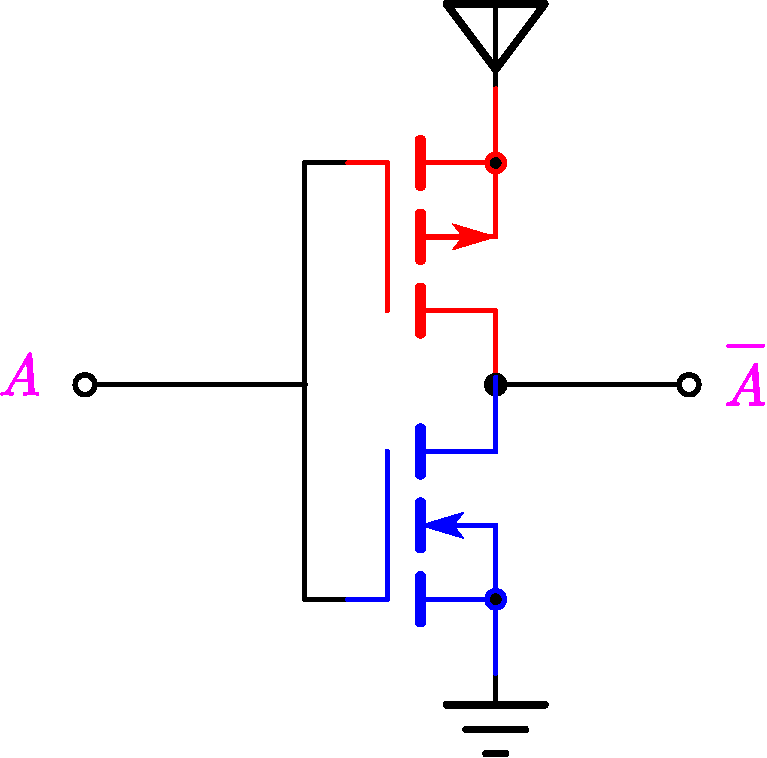
\includegraphics[height=120pt]{assets/5/CMOS NOT.pdf}
        \caption{\bfseries C-MOS NOT }
    \end{subfigure}\hfill
    \begin{subfigure}[t]{0.33\columnwidth}\centering
        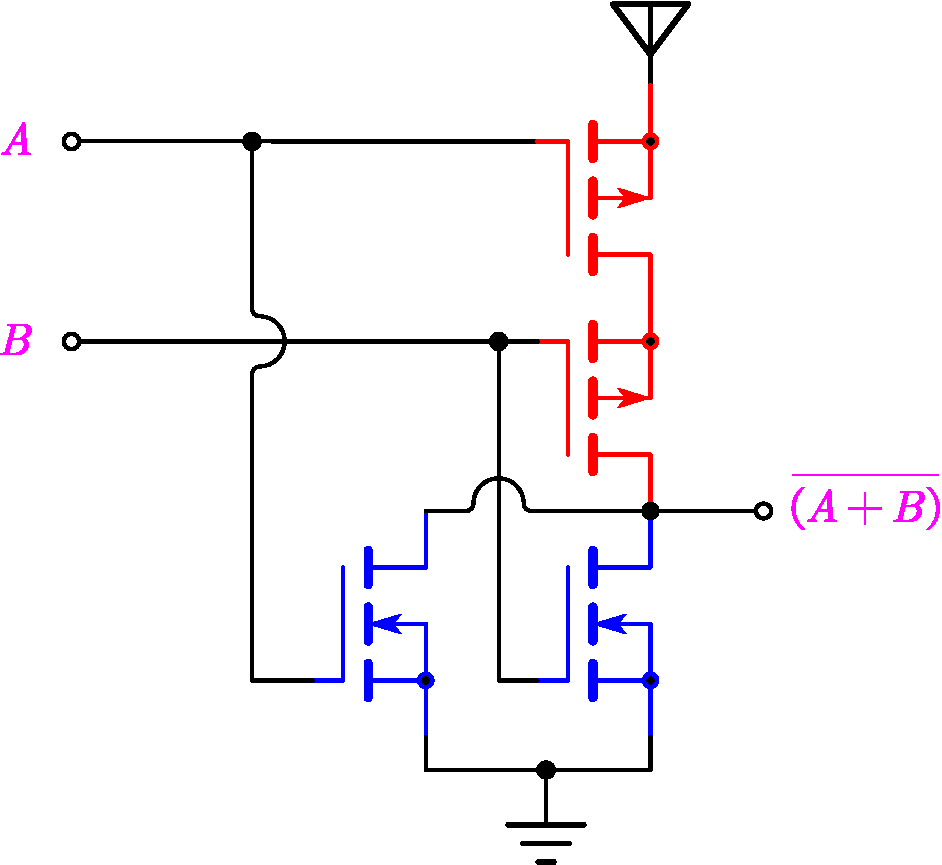
\includegraphics[height=120pt]{assets/5/CMOS NOR.pdf}
        \caption{\bfseries C-MOS NOR }
    \end{subfigure}
    \begin{subfigure}[t]{0.33\columnwidth}\centering
        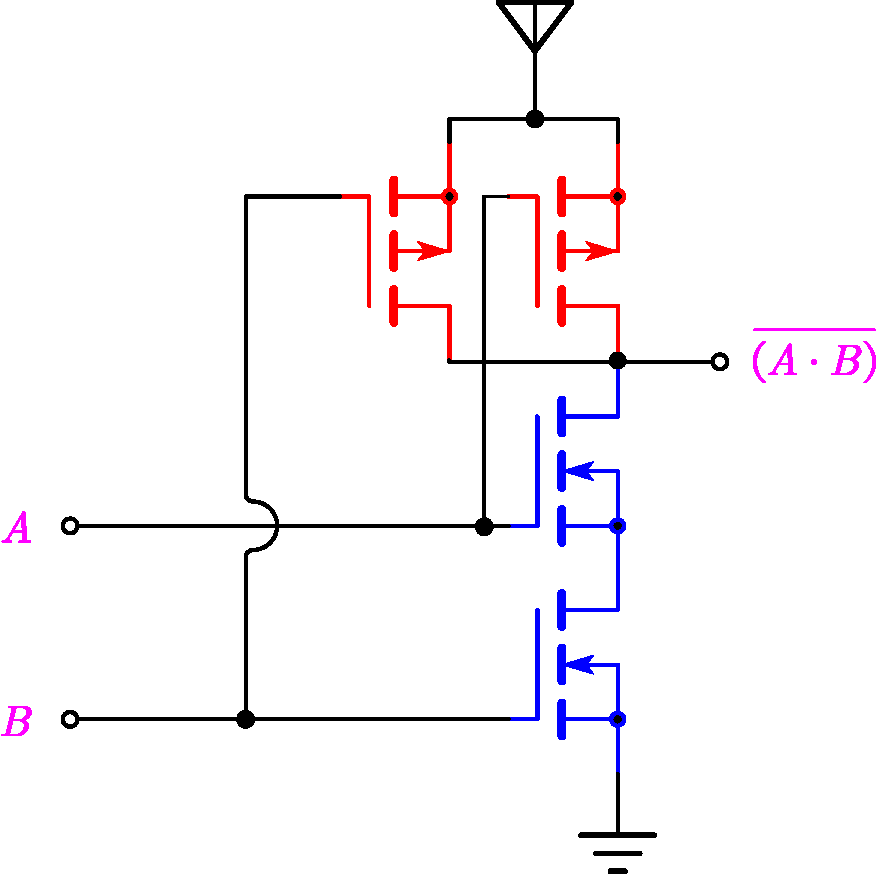
\includegraphics[height=120pt]{assets/5/CMOS NAND.pdf}
        \caption{\bfseries C-MOS NAND }
    \end{subfigure}
    \caption{\bfseries 由 C-MOS 构成三种基本逻辑门 }\label{由 C-MOS 构成三种基本逻辑门}
\end{figure}


\section{半加器、全加器、四位加法器}

\subsection{教材 2-40: 用电源、N-E MOS (最多九个) 和电阻器构成一个半加器 HA}

半加器是一种基本的逻辑电路,用于将两个二进制数相加,输出一个两位的二进制数,表示相加的结果。输出的高位和低位分别称为“进位$C$”、“和位$S$”。也就是说,半加器实际上是“一位加法器”,能够处理两个一位二进制数的相加,并输出一个两位二进制结果。设输入为 $A$ 和 $B$,则有:
\begin{gather}
    Y = (C S)_{(2)} = A_{(2)} + B_{(2)}
    \\
    C = A \cdot B,\quad S = A \oplus B
\end{gather}

由于要求使用的 MOS 尽量少(仅使用 N-MOS),对半加器的逻辑表达式作处理,利用下面式子可得最简半加器(7 个 N-MOS),其数字电路见图 \ref{半加器 HA 数字电路} (a),实际电路见图 \ref{半加器 HA 实际电路} (a)。
\begin{equation}
    C = \overline{(\overline{A\cdot B})},\quad S = \overline{\left[(A \cdot B) + \overline{(A + B)}\right]}
\end{equation}

当然,考虑到半加器的逻辑表达式,也可以用异或门 XOR 和与门 AND 直接构成半加器,我们采用经过优化的 6 MOS 异或门 XOR(三个 N-MOS 和三个 P-MOS),它的静态功率为 0。由此构成的半加器数字电路见图 \ref{半加器 HA 数字电路} (b),实际电路见图 \ref{半加器 HA 实际电路} (b)。

\begin{figure}[H]\centering
\begin{subfigure}[t]{0.5\columnwidth}\centering
    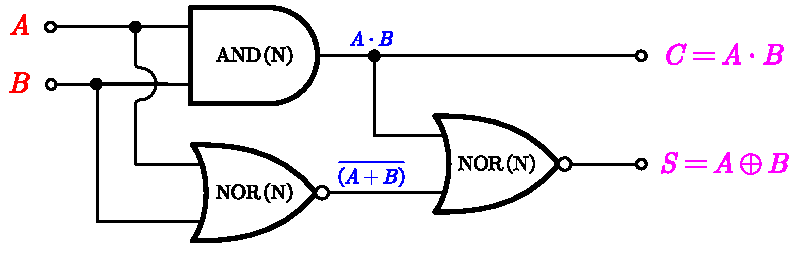
\includegraphics[height=80pt]{assets/5/NMOS 半加器数字电路.pdf}
    \caption{\bfseries N-MOS HA 数字电路}
\end{subfigure}\hfill
\begin{subfigure}[t]{0.5\columnwidth}\centering
    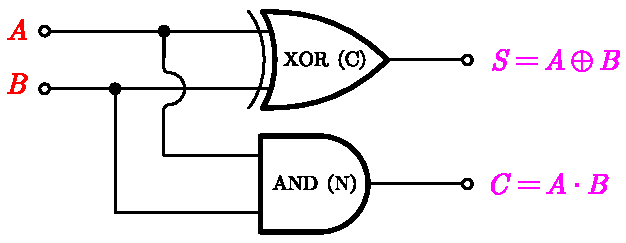
\includegraphics[height=80pt]{assets/5/CMOS 半加器数字电路.pdf}
    \caption{\bfseries C-MOS HA 数字电路 }
\end{subfigure}
\caption{\bfseries 半加器 HA 数字电路 }\label{半加器 HA 数字电路}
\end{figure}

\begin{figure}[H]\centering
\begin{subfigure}[t]{0.42\columnwidth}\centering
    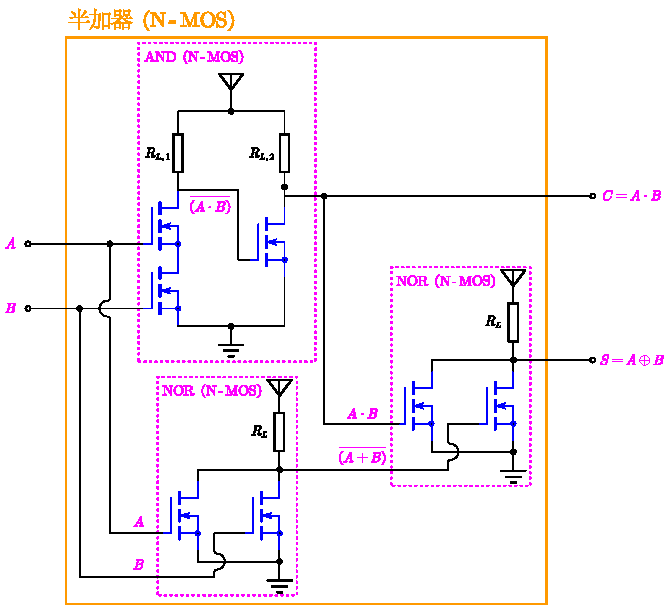
\includegraphics[height=165pt]{assets/5/NMOS 半加器实际电路.pdf}
    \caption{\bfseries N-MOS HA 实际电路 }
\end{subfigure}\hfill
\begin{subfigure}[t]{0.58\columnwidth}\centering
    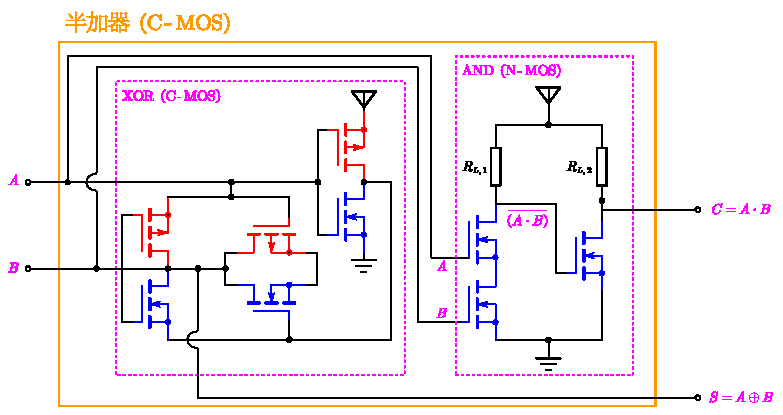
\includegraphics[height=160pt]{assets/5/CMOS 半加器实际电路.pdf}
    \caption{\bfseries C-MOS HA 实际电路 }
\end{subfigure}
\caption{\bfseries 半加器 HA 实际电路 }\label{半加器 HA 实际电路}
\end{figure}

\subsection{用两个半加器 HA 和一个逻辑门构成一个全加器 FA}

由半加器可以进一步构造全加器,全加器是一种能够处理{\color{red} 三个一位二进制数}相加的逻辑电路,输出一个两位的二进制数 $Y= (C_o S)_{(2)}$,表示相加的结果。输出的高位称为进位 $C_o$,低位称为和位 $S$。也就是说,全加器可以理解为“三输入一位加法器”。记全加器的三个输入为 $A$,$B$,$C$,它们都是一位的二进制数,则全加器可写为:
\begin{gather}
Y= (C_oS)_{(2)} = A_{(2)} + B_{(2)} + C_{(2)} 
\\ 
C = A \cdot B + A \cdot C + B \cdot C,\quad 
S = A \oplus B \oplus C
\end{gather}


角标 $(2)$ 表示上式为二进制运算。由两个 HA 和一个 OR 即可构成全加器,数字电路如图 \ref{全加器 FA}。

\begin{figure}[H]\centering
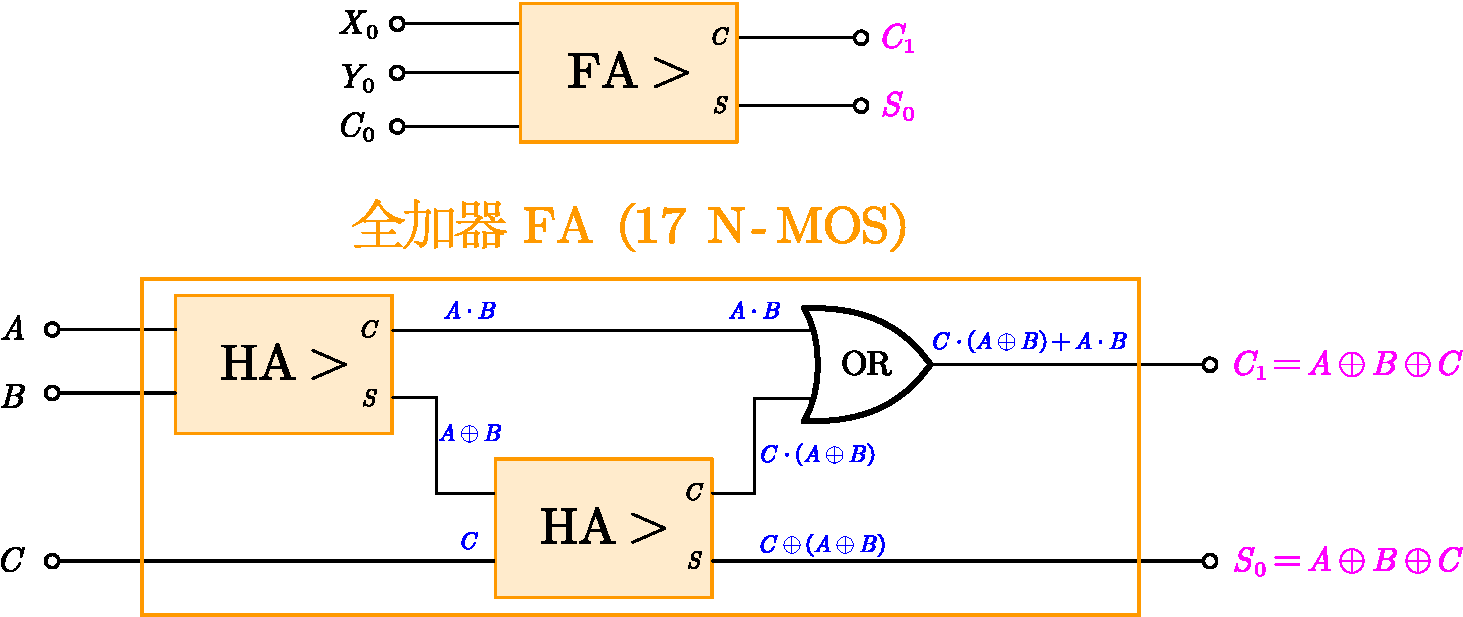
\includegraphics[width=0.65\columnwidth]{assets/5/全加器.pdf}
\caption{\bfseries 全加器 FA}\label{全加器 FA}
\end{figure}



\subsection{用四个全加器 FA 构成一个四位加法器}

四位加法器,输入两个四位二进制数 $X$ 和 $Y$,分别记作 $ X= (X_3 X_2 X_1 X_0)_{(2)}$,$ Y=  (Y_3 Y_2 Y_1 Y_0)_{(2)}$,输出一个五位二进制数 $Z = (C S_3 S_2 S_1 S_0)_{(2)}$,代表两数相加的结果。原理及数字电路如图 \ref{四位加法器} 所示。

\begin{figure}[H]\centering
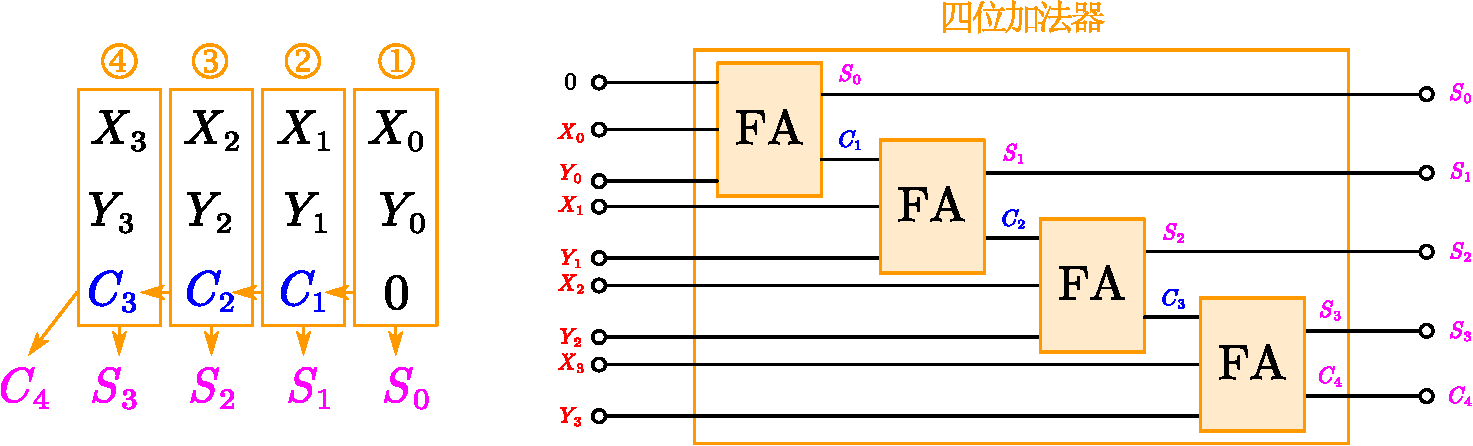
\includegraphics[width=0.9\columnwidth]{assets/5/四位加法器.pdf}
\caption{\bfseries 四位加法器}\label{四位加法器}
\end{figure}


\section{习题集 3-20: 用节点法求图中电路的电流 $I$ 和电流源两端电压 $U$}



对电路作等效处理,得到等效电路如图 \ref{5.4 习题集 3-20} (b) 所示,则有节点电压方程组如下式左半边。再任意选取一个节点作为参考节点,这里选择节点 3,即 $U_3 = 0$,可以解得:
\begin{align}
\begin{cases}
    \text{节点 1: } &  \left(\frac{5}{8} + 1\right)U_1 -  \frac{5}{8} U_2 -  U_3 = - 10.75
    \\
    \text{节点 2: } & - \frac{5}{8} U_1 + \left( \frac{5}{8} + \frac{3}{5}\right)U_2 - \frac{3}{5} U_3 = +10.75 
    \\
    \text{节点 3: } & - U_1 - \frac{3}{5} U_2 + \left(1 + \frac{3}{5}\right)U_3 = 0
\end{cases}
\Longrightarrow 
\begin{bmatrix}
    U_1 \\ 
    U_2 \\
    U_3
\end{bmatrix} 
= 
\begin{bmatrix}
    -\frac{129}{32} \ \mathrm{V}\\
    \frac{215}{32} \ \mathrm{V}\\
    0
\end{bmatrix}
\end{align}

返回到原电路,可得电流 $I$ 和电流源两端电压 $U$: 
\begin{equation}
I = \frac{U_2 - 8 - U_3}{2} = -\frac{41}{64} \ \mathrm{A} = -0.640625 \ \mathrm{A},\quad U = U_2 - U_1 + 6 = \frac{67}{4} \ \mathrm{V} = 16.75 \ \mathrm{V}
\end{equation}

\begin{figure}[H]\centering
\begin{subfigure}[t]{0.5\columnwidth}\centering
    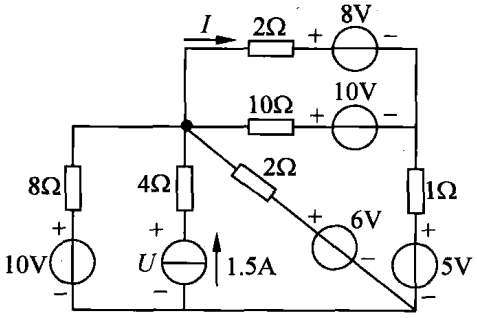
\includegraphics[height=120pt]{assets/5/5.4 (1).png}
    \caption{\bfseries 题目原电路图 }
\end{subfigure}\hfill
\begin{subfigure}[t]{0.5\columnwidth}\centering
    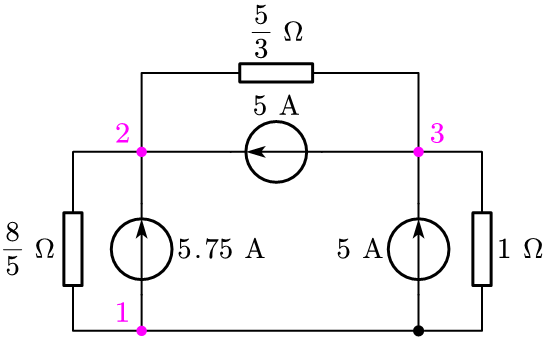
\includegraphics[height=120pt]{assets/5/5.4 (2).png}
    \caption{\bfseries 等效后的最简电路图 }
\end{subfigure}
\caption{\bfseries 5.4 习题集 3-20 }\label{5.4 习题集 3-20}
\end{figure}


\section{习题集 3-21: 用节点法求电流源两端电压 $U$ 和各支路电流 }

还是对电路作等效处理,得到等效电路如图 \ref{5.5 习题集 3-21} (b) 所示。这次先选取参考节点再列方程,以节点 0 为参考点,得到:
\begin{equation}
\left(\frac{1}{13.7} + \frac{1}{17.2} + \frac{1}{11.9}\right) U_1 = \frac{5}{13.7} + \frac{15}{17.2} + \frac{10}{11.9} + 1\Longrightarrow U_1 = 14.3024 \ \mathrm{V}
\end{equation}
% \Longrightarrow  0.21517U_1 = 3.07739
于是得到电压 $U$ 和各支路电流:
\begin{align}
U = U_1 + 5.5 = 19.8024 \ \mathrm{V} ,\quad  
I_1 = \frac{U_1 - 5}{13.7} =  0.6790 \ \mathrm{A}\\ 
I_2 = \frac{U_1 - 15}{17.2} = -0.0406 \ \mathrm{A}, \quad 
I_3 = \frac{U_1 - 10}{11.9} = 0.3615 \ \mathrm{A}
\end{align}


\begin{figure}[H]\centering
\begin{subfigure}[t]{0.5\columnwidth}\centering
    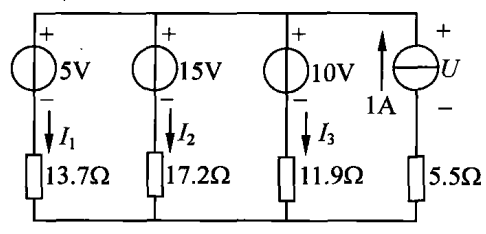
\includegraphics[height=120pt]{assets/5/5.5 (1).png}
    \caption{\bfseries 题目原电路图 }
\end{subfigure}\hfill
\begin{subfigure}[t]{0.5\columnwidth}\centering
    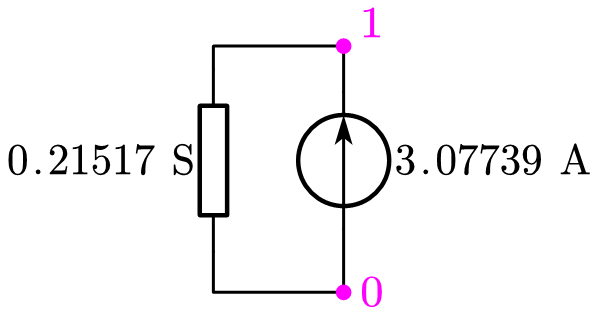
\includegraphics[height=120pt]{assets/5/5.5 (2).png}
    \caption{\bfseries 等效后的最简电路图 }
\end{subfigure}
\caption{\bfseries 5.5 习题集 3-21 }\label{5.5 习题集 3-21}
\end{figure}


\section{(选做)讲义题 3-4: 按指定的参考节点,列出电路的节点电压方程}

原题图和等效电路如图 \ref{5.6 讲义题 3-4} 所示,电路中有 4 个节点(不含无伴电压源)和 2 个受控源控制变量,需要列出 3 个节点方程和 2 个控制方程,如下:
\begin{align}
\begin{matrix}
    \text{节点 1: } & (1 + 1)U_1 - U_2 - 0 = 2u-1\\
    \text{节点 2: } & -U_1 + \left(1 + \frac{1}{4}\right)U_2 - \frac{1}{4}U_3 = 3 i  \\
    \text{节点 3: } &  0-\frac{1}{4}U_2 + \left(1 + \frac{1}{4}\right)U_3 = 1 \\
    \text{控制方程: } & i = U_1 - U_2,\quad u = U_3
\end{matrix}
\end{align}
代入化简并求解:
\begin{equation}
\begin{cases}
    2U_1 - U_2 -2 U_3 = -1\\ 
    -16U_1 + 17U_2 - U_3 = 0 \\ 
    0 - U_2 + 5U_3 = 1
\end{cases}\Longrightarrow 
U_1 = U_2 = U_3 = 1 \ \mathrm{V},\quad i = 0,\quad u = 1 \ \mathrm{V}
\end{equation}

\begin{figure}[H]\centering
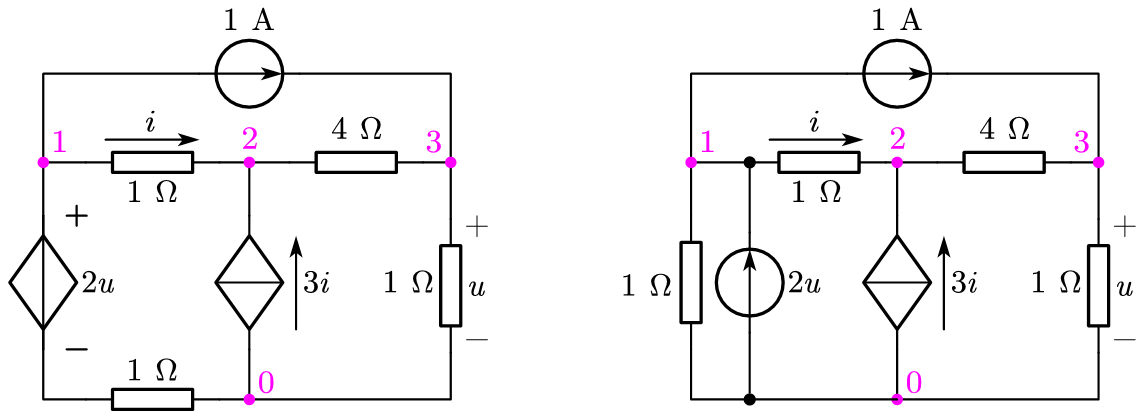
\includegraphics[width=0.8\columnwidth]{assets/5/5.6.png}
\caption{\bfseries 5.6 讲义题 3-4}\label{5.6 讲义题 3-4}
\end{figure}

\section{习题集 3-15: 用回路电流法求图中电路的独立电流源功率}

原电路已无法继续化简,电路中有 3 个网格(含 2 个无伴电流源),1 个受控源变量,共需列出 $3 + 1 = 2$ 个方程。如图 \ref{5.7 习题集 3-15} (a),先列出三个网格电流方程,如下:
\begin{align}
    \text{网格 1: } & 100 i_1 - 20i_2 - 30i_3 = 0 \\ 
    \text{网格 2: } & i_2 = 1 \\ 
    \text{网格 3: } & i_3 = -0.02 U
\end{align}
又有控制变量 $U$: 
\begin{equation}
0 + U - 20(i_2 - i_1) - 0.4 U = 0 \Longrightarrow U = \frac{100}{3}(i_2 - i_1)
\end{equation}
联立上面四个方程,可以得到:
\begin{equation}
\begin{cases}
    \text{网格 1: } & 100 i_1 - 20i_2 - 30i_3 = 0 \\ 
    \text{网格 2: } & i_2 = 1 \\ 
    \text{网格 3: } & -2 i_1 + 2i_2 +3 i_3 = 0
\end{cases}
\Longrightarrow 
\begin{cases}
    i_1 = 0 \ \mathrm{A} \\ 
    i_2 = 1 \ \mathrm{A} \\ 
    i_3 = -\frac{2}{3} \ \mathrm{A}
\end{cases}
\end{equation}
得到功率 $P$:
\begin{equation}
    P = 1 \ \mathrm{A}\cdot U = \frac{100}{3}(i_2 - i_1) = \frac{100}{3} \ \mathrm{W} = 33.3333 \ \mathrm{W}
\end{equation}

\begin{figure}[H]\centering
\begin{subfigure}[t]{0.5\columnwidth}\centering
    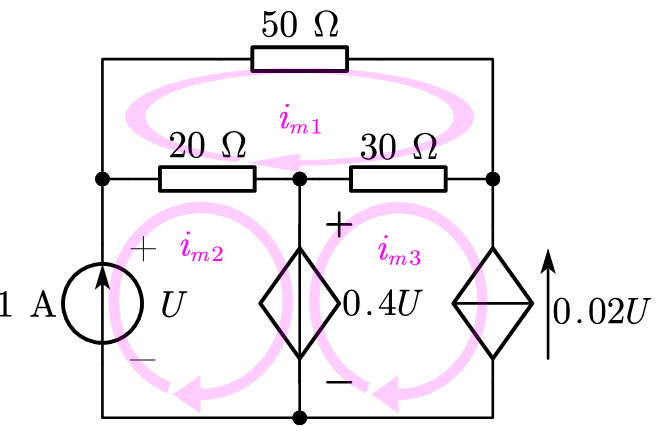
\includegraphics[height=120pt]{assets/5/5.7 (1).png}
    \caption{\bfseries 回路电流法 }
\end{subfigure}\hfill
\begin{subfigure}[t]{0.5\columnwidth}\centering
    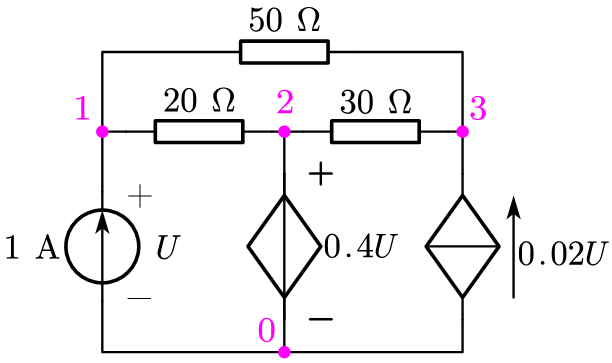
\includegraphics[height=120pt]{assets/5/5.7 (2).png}
    \caption{\bfseries 节点电压法 }
\end{subfigure}
\caption{\bfseries 5.7 习题集 3-15 }\label{5.7 习题集 3-15}
\end{figure}

不妨也用节点电压法求解一下此题。如图 \ref{5.7 习题集 3-15} (b),电路中有 4 个节点(含 1 个无伴电压源)和 1 个(受控源)控制变量,取节点 0 为参考节点,共需列出 $ (4 - 1 - 1) + 0 + 2 = 4$ 个方程,如下:
\begin{align}
\text{节点 1: } & \left(\frac{1}{50} + \frac{1}{20}\right) U_1 - \frac{1}{20}U_2 - \frac{1}{50}U_3 = 1 \\ 
\text{节点 2: } & U_2 = 0.4 U \\
\text{节点 3: } & - \frac{1}{50}U_1 - \frac{1}{30}U_2 + \left(\frac{1}{50} + \frac{1}{30}\right)U_3 = 0.02 U \\ 
\text{控制方程: } & U = U_1
\end{align}
联立上述四个方程,可以得到:
\begin{equation}
\begin{cases}
    \text{节点 1: } & \left(\frac{1}{50} + \frac{1}{20}\right) U_1 - \frac{1}{20}U_2 - \frac{1}{50}U_3 = 1 \\ 
    \text{节点 2: } & -0.4 U_1 + U_2 = 0 \\
    \text{节点 3: } & - \frac{2}{50}U_1 - \frac{1}{30}U_2 + \left(\frac{1}{50} + \frac{1}{30}\right)U_3 = 0
\end{cases}
\Longrightarrow 
\begin{cases}
    U_1 = \frac{100}{3} \ \mathrm{V}\\ 
    U_2 = \frac{40}{3} \ \mathrm{V}\\ 
    U_3 = \frac{100}{3} \ \mathrm{V}
\end{cases}
\Longrightarrow P = 1 \ \mathrm{A}\cdot U = \frac{100}{3} \ \mathrm{W}
\end{equation}

\section{(选做)讲义题 3-8: 列出图中电路的网孔电流方程,并计算受控源的吸收功率}

如图,电路共有 3 个网格(内含 2 个无伴电流源)和 1 个控制变量,将 $i_2$ 和 $i_3$ 合并为超网格后,共需要列出 2 个网格方程、1 个超网格内部方程和 1 个控制方程,如下:
\begin{equation}
\begin{cases}
    \text{网格 1: } & i_1 = 2\\ 
    \text{网格 2,3: } & -3i_1 + (2i_2 + 4i_3) = 4\\ 
    \text{网格 2,3 内部: } & 2i = i_2 - i_3\\ 
    \text{控制方程: } & i = i_3 - i_1
\end{cases}\Longrightarrow 
\begin{cases}
    i_1 = 2 \\ 
    -3i_1 + 2i_2 + 4i_3 = 4 \\
    2i_1 + i_2 - 3i_3 = 0
\end{cases}
\Longrightarrow 
\begin{cases}
    i_1 = 2 \ \mathrm{A}\\ 
    i_2 = 1.4 \ \mathrm{A}\\ 
    i_3 = 1.8 \ \mathrm{A} \\ 
    i = -0.2 \ \mathrm{A}
\end{cases}
\end{equation}
于是得到吸收功率:
\begin{equation}
    P = 2i \cdot \left[ 0 - \left(4 - 2(i_2 - i_1)\right) \right] = 2.8 \ \mathrm{W}
\end{equation}

\begin{figure}[H]\centering
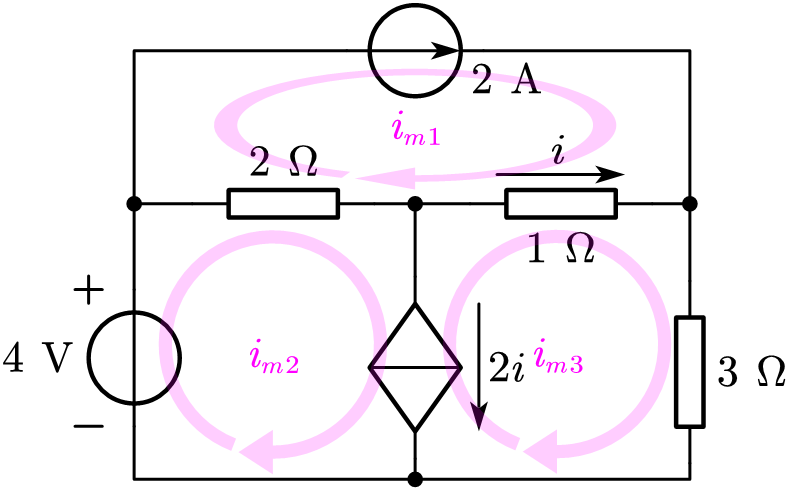
\includegraphics[width=0.5\columnwidth]{assets/5/5.8.png}
\caption{\bfseries 5.8 讲义题 3-8}\label{5.8 讲义题 3-8}
\end{figure}


\chapter{Homework 6: 2024.10.9 - 2024.10.15}\thispagestyle{fancy}

\section{习题集 4-10: 题图电路中电流源 $I_{S1} = 2 \ \mathrm{A}$,$I_{S2}= 3 \ \mathrm{A}$。断开 3 A 电流源,则 2 A 电流源输出 28 W,$U$ = 8 V。断开 2 A 电流源,则 3 A 的电流源输出 54 W,$U$ = 12 V。求两个电流源同时作用时,每个电流源输出的功率。}

仅有 $2 \ \mathrm{A}$ 电流源时,$U_1 = 14 \ \mathrm{V}$,$U_2 = 8 \ \mathrm{V}$;仅有 $3 \ \mathrm{A}$ 电流源时,$U_1 = 12 \ \mathrm{V}$,$U_2 = 18 \ \mathrm{V}$。由叠加定理,两电流源同时作用时:
\begin{equation}
\begin{cases}
    U_1 = 14 + 12 = 26 \ \mathrm{V} \\ 
    U_2 = 8 + 18 = 26 \ \mathrm{V}
\end{cases}
\Longrightarrow 
\boxed{
    \begin{cases}
        P_{2\mathrm{A}} = 2 \cdot 26 = 52 \ \mathrm{W} \\ 
        P_{3\mathrm{A}} = 3 \cdot 26 = 78 \ \mathrm{W}
    \end{cases}
}
\end{equation}
\begin{figure}[H]\centering
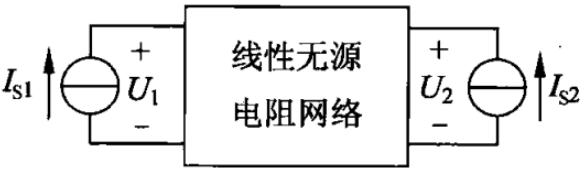
\includegraphics[width=0.4\columnwidth]{assets/6/9506aa8f7aeba32072fee006fa1076c7.png}
\caption{\bfseries 6.1 习题集 4-10}\label{6.1 习题集 4-10}
\end{figure}

\section{习题集 4-24: 题图电路中,已知 $U_{S1} = 24 \ \mathrm{V},\  U_{S2} = 18 \ \mathrm{V},\ R_1 = 2 \ \Omega,\ R_2 = 1 \ \Omega,\ R_3 = 3 \ \Omega$。}

\subsection{求 $U_{S3} = 15 \ \mathrm{V}$ 时,通过 $R_3$ 的电流}

先求出激励为单个电压源时,通过 $R_3$ 的电流(参考方向标在图 \ref{6.2 习题集 4-24} 中):
\begin{equation}
U_{S1}:\ I_{R_3} = \frac{24}{11} \ \mathrm{A} ,\quad U_{S2}:\ I_{R_3} = -\frac{36}{11} \ \mathrm{A},\quad U_{S3}:\ I_{R_3} = \frac{3}{11} U_{S3}
\end{equation}
由叠加定理,通过 $R_3$ 的电流为:
\begin{equation}
\boxed{
    I_{R_3} = \frac{24}{11} - \frac{36}{11} + \frac{3}{11} \cdot 15 = 3 \ \mathrm{A}
}
\end{equation}

\begin{figure}[H]\centering
\begin{subfigure}[t]{0.55\columnwidth}\centering
    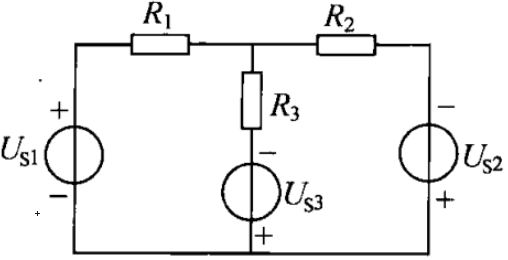
\includegraphics[height=115pt]{assets/6/a45e47a606698b8a935641ad6e1e5ab9.png}
    \caption{\bfseries 原题图 }
\end{subfigure}\hfill
\begin{subfigure}[t]{0.45\columnwidth}\centering
    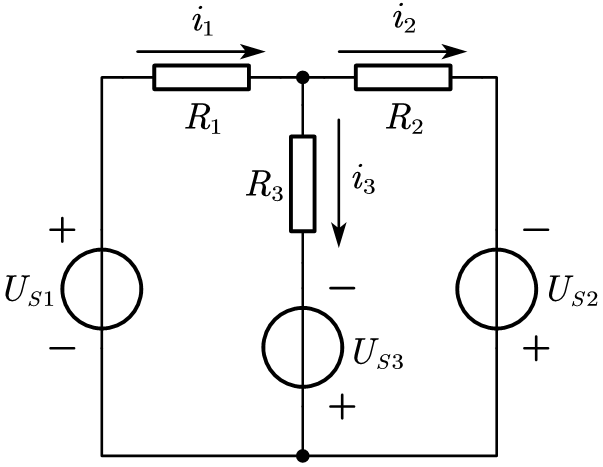
\includegraphics[height=125pt]{assets/6/0d7f9f1c42f022fbf24925b67ee966d3.png}
    \caption{\bfseries 电流参考方向 }
\end{subfigure}
\caption{\bfseries 6.2 习题集 4-24}\label{6.2 习题集 4-24}
\end{figure}

\subsection{$R_3$ 为多大时可获得最大功率,值是多少}

此题表述有些问题,既没有说明固定 $U_{S3}$ 的值为多少,也没有强调“功率”的主语,是指“$R_3$ 的功率”还是“电路总功率”,有些模糊不清。不论功率是前者还是后者,必须先给定 $U_{S3}$ 才可计算。所以,我们在这里沿用第一问的条件,假设 $U_{S1} = 15 \ \mathrm{V}$,则各电源(激励)对电阻的电流为:
\begin{align}
    U_{S1}:\quad & 
    I_{R_1} = \frac{U_{S1}}{R_1 + R_2 \parallel R_3},\quad 
    I_{R_2} = I_{R_1}\cdot \frac{R_3}{R_2 + R_3},\quad 
    I_{R_3} = I_{R_1}\cdot \frac{R_2}{R_2 + R_3} \\ 
    U_{S2}:\quad & 
    I_{R_1} =  I_{R_2}\cdot \frac{R_3}{R_1 + R_3},\quad 
    I_{R_2} =\frac{U_{S2}}{R_2 + R_1 \parallel R_3},\quad  
    I_{R_3} = - I_{R_2}\cdot \frac{R_1}{R_1 + R_3} \\ 
    U_{S3}:\quad & 
    I_{R_1} =  I_{R_3}\cdot \frac{R_2}{R_1+ R_2},\quad 
    I_{R_2} = - I_{R_3}\cdot \frac{R_1}{R_1 + R_2} ,\quad 
    I_{R_3} = \frac{U_{S3}}{R_3 + R_1 \parallel R_2}
\end{align}
由叠加定理计算 $R_3$ 的功率和电路总功率:
\begin{equation}
    P_{R_3} = I_{R_3}^2R_3,\quad P = I_{R_1}^2R_1 + I_{R_2}^2R_2 + I_{R_3}^2R_3
\end{equation}
代入数据,做数学上的化简和整理,可得:
\begin{equation}
    P_{R_3} = \frac{1089 R_3}{(3 R_3 + 2)^2} = \frac{1089}{9 R_3 + \frac{4}{R_3} + 12} ,\quad P = \frac{363}{3R_3 + 2 } + 588
\end{equation}
于是:
\begin{center}
    \boxed{
        \begin{matrix}
            \text{
                当 $R_3 = \frac{2}{3} \Omega$ 时,$R_3$ 有最大功率 $P_{R_3, \max} = \frac{363}{8} \ \mathrm{W} = 45.375 \ \mathrm{W}$
            }\\ 
            \text{
                当 $R_3 = 0$ 时,有最大电路总功率 $P_{\max} = \frac{1539}{2} \ \mathrm{W} = 769.5 \ \mathrm{W}$
            }
        \end{matrix}
        }
\end{center}

%\begin{align}
%    U_{S1}:\quad & 
%    I_{R_1} = \frac{96}{11}\ \mathrm{A},\quad 
%    I_{R_2} = \frac{72}{11}\ \mathrm{A},\quad 
%    I_{R_3} = \frac{24}{11} \ \mathrm{A} 
%    \\
%    U_{S2}:\quad & 
%    I_{R_1} = \frac{54}{11}\ \mathrm{A},\quad 
%    I_{R_2} = \frac{90}{11}\ \mathrm{A},\quad 
%    I_{R_3} = -\frac{36}{11} \ \mathrm{A} 
%    \\
%    U_{S3}:\quad & 
%    I_{R_1} = \frac{1}{11}U_{S3},\quad 
%    I_{R_2} = -\frac{2}{11}U_{S3},\quad
%    I_{R_3} = \frac{3}{11} U_{S3}
%\end{align}




\subsection{求使 $R_3$ 中电流为 0 的 $U_{S3}$}

由叠加定理:
\begin{equation}
\boxed{
    \frac{24}{11} - \frac{36}{11} + \frac{3}{11} \cdot U_{S3} = 0 \Longrightarrow U_{S3} = 4 \ \mathrm{V}
}
\end{equation}

\section{习题集 4-36: 题图电路中网络 $A$ 内含有独立电压源、电流源和线性电阻。在 (a) 图中测得 $U_{ab} = 10 \ \mathrm{V}$,(b) 图中测得 $U_{a'b'} = 4 \ \mathrm{V}$,求 (c) 图中的电压 $U_{a''b''}$。}

由戴维南定理,可将网络 $A$ 等效为一个电压源 $U$ 串联一个电阻 $R$,如图 \ref{6.3 习题集 4-36.2} (a) 所示。列出方程:
\begin{equation}
U = 10 - 0.5 R,\quad U - 0.4 R = 4 \Longrightarrow R = \frac{20}{3} \ \Omega,\quad U = \frac{20}{3} \ \mathrm{V}
\end{equation}
作电源等效如图 \ref{6.3 习题集 4-36.2} (b),求得题图 (c) 中的 $U_{a''b''}$:
\begin{equation}
R_0 = R \parallel 10 \ \Omega \parallel 8 \ \Omega = \frac{8}{3} \ \Omega,\quad I_0 = \frac{U}{R} + 0.5 + 1 = 2.5 \ \mathrm{A} \Longrightarrow 
\boxed{
    U_{a''b''} =  I_0R_0 = \frac{20}{3} \ \mathrm{V} = 6.67 \ \mathrm{V}
}
\end{equation}

\begin{figure}[H]\centering
\includegraphics[width=0.85\columnwidth]{assets/6/image (7).jpg}
\caption{\bfseries 6.3 习题集 4-36}\label{6.3 习题集 4-36}
\end{figure}

\begin{figure}[H]\centering
\begin{subfigure}[t]{0.6\columnwidth}\centering
    \includegraphics[height=100pt]{assets/6/acd560ff4ae20eb901019a90b84ef837.png}
    \caption{\bfseries 戴维南定理等效 }
\end{subfigure}\hfill
\begin{subfigure}[t]{0.4\columnwidth}\centering
    \includegraphics[height=100pt]{assets/6/7367192b138adaf93ddf5c5fcc94a53b.png}
    \caption{\bfseries 等效电源 }
\end{subfigure}
\caption{\bfseries 6.3 习题集 4-36 的等效处理}\label{6.3 习题集 4-36.2}
\end{figure}

\section{习题集 4-37: 题图电路方框内为线性电阻网络,测得 $U_S = 8 \ \mathrm{V},\ R = 3 \ \Omega$ 时 $I = 0.5 \ \mathrm{A}$;$U_S = 18 \ \mathrm{V},\ R = 4 \ \Omega$ 时 $I = 1 \ \mathrm{A}$。求 $U_S = 30 \ \mathrm{V},\ R = 5 \ \Omega$ 时的电流 $I$。}

由戴维南定理,将方框内的线性电阻网络与电压源 $U_S$ 等效为一个电压源 $U_0$ 串联一个电阻 $R_0$,如图 \ref{6.4 习题集 4-37} 所示。当 $U_S$ 从 $8 \ \mathrm{V}$ 变为 $18 = \frac{9}{4} \cdot 8\ \mathrm{V}$ 时,由齐性定理,等效后的电压源 $U_0$ 应变为 $\frac{9}{4}U_0$,于是可求得 $U_0$ 和 $R_0$:
\begin{equation}
\begin{cases}
    U_0 = 0.5 (R_0 + 3)\\ 
    \frac{9}{4}U_0 =  R_0 + 4
\end{cases} 
\Longrightarrow 
\begin{cases}
    R_0 = 5 \Omega \\ 
    U_0 = 4 \ \mathrm{V}
\end{cases}
\Longrightarrow 
\boxed{
    I\mid_{R = 5 \Omega} = \left[\frac{ \frac{30}{8} U_0}{R_0 + R}\right]_{R = 5 \Omega} = 1.5 \ \mathrm{A}
}
\end{equation}

\begin{figure}[H]\centering
\includegraphics[width=0.52\columnwidth]{assets/6/0f2c149b099f73467b72503826e5385d.png}
\caption{\bfseries 6.4 习题集 4-37}\label{6.4 习题集 4-37}
\end{figure}

\section{(选做)讲义题 3-13: 题图电路中,$R_x = 0$ 时测得 $I_x = 8 \ \mathrm{A}$,$U = 12 \ \mathrm{V}$;$R_x = \infty$ 时测得 $U_x = 36 \ \mathrm{V}$,$U = 6 \ \mathrm{V}$。求出 $R_x = 9 \ \Omega$ 时的 $U_x$ 和 $U$。}

先将除 $R_x$ 外的电路等效为戴维南电路,设戴维南电路的电压源为 $U_1$,电阻为 $R_1$,由题意可得:
\begin{equation}
\begin{cases}
    U_1 = 36 \ \mathrm{V} \\ 
    R_1 = \frac{36}{8} \ \Omega = 4.5 \ \Omega
\end{cases}
\Longrightarrow 
\boxed{
    U_x \mid_{R_x = 9 \Omega} = U_1 \cdot \frac{R_x}{R_1 + R_x} = 24 \ \mathrm{V}
}
\end{equation}

然后用替代定理,将 $R_x$ 替换为电压源 $U_x$。由叠加定理和齐性定理,可得:
\begin{equation}
    U = U' + kU_x
    \Longrightarrow 
\begin{cases}
    U' = 12 \ \mathrm{V} \\ 
    6 = 12 + k \cdot 36
\end{cases}
\Longrightarrow 
\begin{cases}
    U' = 12 \ \mathrm{V} \\ 
    k = -\frac{1}{6}
\end{cases}
\Longrightarrow 
\boxed{
    U\mid_{R_x = 9 \Omega} = 12 - \frac{1}{6} \cdot 24 = 8 \ \mathrm{V}
}
\end{equation}

\begin{figure}[H]\centering
\begin{subfigure}[t]{0.45\columnwidth}\centering
    \includegraphics[height=125pt]{assets/6/image (9).jpg}
    \caption{\bfseries 讲义 3-13 题图 }
\end{subfigure}\hfill
\begin{subfigure}[t]{0.55\columnwidth}\centering
    \includegraphics[height=125pt]{assets/6/image (10).jpg}
    \caption{\bfseries 讲义 3-18 题图 }
\end{subfigure}
\caption{\bfseries 讲义题 3-13、讲义题 3-18 }
\end{figure}

\section{(选做)讲义题 3-18: 题图电路中 OPA 理想,求 ab 端口的诺顿等效电路,以及电流之比 $\frac{i_1}{i_4}$(设ab端开路)。}

由虚短和虚断,$i_4 = - \frac{u_s}{R_2} \Longrightarrow U_{ab} = -\frac{R_4}{R_2}u_s$,将电压源置零,可得戴维南等效电阻为 $R = R_4$,于是诺顿等效电流为 $i = \frac{U}{R} = - \frac{u_s}{R_2}$,也即大小 $\frac{u_s}{R_2}$,由 $a$ 指向 $b$,如图 \ref{6.6 等效电路、6.7 题图} (a) 所示。并且电流之比:
\begin{equation}
u_s - i_1R_1 = \left(1 - \frac{R_3 + R_4}{R_2}u_s\right) \Longrightarrow  \boxed{
    \frac{i_1}{i_4} = - \frac{R_3 + R_4}{R_2}
}
\end{equation}

\begin{figure}[H]\centering
\begin{subfigure}[t]{0.5\columnwidth}\centering
    \includegraphics[height=120pt]{assets/6/9d53a9b244bf76e6ad1734869043135a.png}
    \caption{\bfseries 6.6 讲义题 3-18 诺顿等效电路 }
\end{subfigure}\hfill
\begin{subfigure}[t]{0.5\columnwidth}\centering
    \includegraphics[height=120pt]{assets/6/2e96a177467ade2ca35ed590fb9751d7.png}
    \caption{\bfseries 6.7 习题集 4-47 }
\end{subfigure}
\caption{\bfseries 6.6 等效电路、6.7 题图 }\label{6.6 等效电路、6.7 题图}
\end{figure}

\section{习题集 4-47: 图 \ref{6.6 等效电路、6.7 题图} (b) 中,N 为纯电阻网络,已知 $ab$ 端开路电压 $U_o = 8 \ \mathrm{V}$,$ab$ 端纽左端的戴维南等效电阻 $R = 3 \ \Omega$,电压源 $U_S = 10 \ \mathrm{V}$。若 $ab$ 两端接上 $R_L = 2 \ \Omega$ 电阻时,电压源 $U_S$ 供出电流 $I_1$。求当把 $R_L$ 移走之后,电流 $I_1$ 变化多少?} 

由特勒根定理,设电路总支路数为 $b$,由特勒根定理:
\begin{equation}
\sum_{k = 1}^{2} u_k \hat{i}_k + \sum_{k = 3}^{b} u_k \hat{i}_k =  0 = \sum_{k = 1}^{2} \hat{u}_k i_k + \sum_{k = 3}^{b} \hat{u}_k i_k 
\end{equation}
其中支路 $3 \sim b$ 是网络 N 内部的支路,由于 $N$ 为纯电阻网络,有:
\begin{equation}
    \sum_{k = 3}^{b} u_k \hat{i}_k  = \sum_{k = 3}^{b} i_k R_k \hat{i}_k =  \sum_{k = 3}^{b} \hat{u}_k i_k 
\end{equation}
于是内部项可以消去,得到:
\begin{gather}
    u_1\hat{i}_1 + u_2 \hat{i}_2 = \hat{u}_1i_1 + \hat{u}_2 i_2 \Longrightarrow 
U_S I_1' + 0 = U_SI_1 + U_o \frac{U_o}{R_L + R}
\Longrightarrow \\
\boxed{
    \Delta I_1 = \frac{U_o}{U_S}\cdot\frac{U_o}{R_L + R} = 1.28 \ \mathrm{A}
}
\end{gather}


\section{(选做)讲义题 3-20: 题图电路中,$N_R$ 为只含线性电阻的网络,试求解电压 $U_R$。}

$N_R$ 为线性电阻网络,由互易定理:
\begin{equation}
    u_1\hat{i}_1 + u_2 \hat{i}_2 = \hat{u}_1i_1 + \hat{u}_2 i_2 \Longrightarrow 
    10\cdot \left(- \frac{U_R}{2}\right) + 0 = U_R\cdot 5 + 10 \cdot 1 \Longrightarrow \boxed{
        U_R = -1 \ \mathrm{V}
    }
\end{equation}


\begin{figure}[H]\centering
\begin{subfigure}[t]{0.5\columnwidth}\centering
    \includegraphics[height=120pt]{assets/6/940731df99ca203c28371281cebfb9ca.png}
\end{subfigure}\hfill
\begin{subfigure}[t]{0.5\columnwidth}\centering
    \includegraphics[height=120pt]{assets/6/7c27b6b5231748eb023412fd0cbe700c.png}
\end{subfigure}
\caption{\bfseries 6.8 讲义题 3-20 }
\end{figure}










































% --------------------------- 仿真作业 --------------------------- %
% >> ------------------------ 仿真作业 ------------------------ << %


\chapter{Simulate 1: 2024.9.10 - 2024.9.24}
\lhead{Simulate 1: 2024.9.10 - 2024.9.24}
\thispagestyle{fancy}

\section{仿真 2-1: 题目详见图 \ref{示意图} (b)}

\subsection{单 OPA 实现电压运算}

电路如图 \ref{单 OPA 实现 电压运算} (a) 所示,接线端示意图见图 \ref{单 OPA 实现 电压运算} (b)。

\begin{figure}[H]\centering
\begin{subfigure}[t]{0.43\textwidth}\centering
    \includegraphics[height=150pt]{assets/3/单OPA.png}
    \caption{\bfseries 电路示意图 }
\end{subfigure}\begin{subfigure}[t]{0.43\textwidth}\centering
    \includegraphics[height=150pt]{assets/3/单OPA接线端.png}
    \caption{\bfseries 接线端示意图 }
\end{subfigure}
\caption{\bfseries 单 OPA 实现 电压运算 }\label{单 OPA 实现 电压运算}
\end{figure}

下面分析其输出特性。由虚断,在 $u_1$ 和 $u_2$ 构成的回路中,设正向流经 $u_2$ 的电流为 $i_2$,则有:
\begin{equation}
i_2 = \frac{u_2 - u_1}{R_1+R_2}
\Longrightarrow  
u_A = u_2 - i_2R_2 = \frac{R_2u_1 + R_1u_2}{R_1 + R_2}
\end{equation}
由虚短,B 点的电势也为 $u_A$,于是:
\begin{equation}
i_3 = \frac{u_3 - u_A}{R_3},\ i_M = \frac{u_A}{R_M} \Longrightarrow  i_f = i_3 - i_M = \frac{u_3 - u_A}{R_3} - \frac{u_A}{R_M} = \frac{u_3}{R_3} - (\frac{1}{R_3} + \frac{1}{R_M})u_A
\end{equation}
由虚断和 KVL:
\begin{equation}
u_o = u_A - i_fR_f = u_A - \frac{R_f}{R_3}u_3 + (\frac{R_f}{R_3} + \frac{R_f}{R_M})u_A = \left( 1 +  \frac{R_f}{R_3} + \frac{R_f}{R_M}\right)u_A - \frac{R_f}{R_3}u_3
\end{equation}
将 $u_A$ 的表达式代入,最终得到:
\begin{equation}
\boxed{
    u_o = \left( 1 +  \frac{R_f}{R_3} + \frac{R_f}{R_M}\right)\frac{1}{\frac{R_1}{R_2} + 1}u_1 
    + \left( 1 +  \frac{R_f}{R_3} + \frac{R_f}{R_M}\right)\frac{\frac{R_1}{R_2}}{\frac{R_1}{R_2} + 1}u_2
    - \frac{R_f}{R_3}u_3
}
\end{equation}
我们需要 $u_1,u_2,u_3$ 前的系数分别为 3, 2, -0.5,于是有:
\begin{equation}
\begin{cases}
    \left( 1 +  \frac{R_f}{R_3} + \frac{R_f}{R_M}\right)\frac{1}{\frac{R_1}{R_2} + 1} = 3 \vspace*{5pt}\\ 
    \vspace*{5pt}
    \left( 1 +  \frac{R_f}{R_3} + \frac{R_f}{R_M}\right)\frac{\frac{R_1}{R_2}}{\frac{R_1}{R_2} + 1} = 2 \\ 
    -\frac{R_f}{R_3} = -0.5
\end{cases}
\Longrightarrow 
\begin{cases}
    R_1 = \frac{2}{3}R_2 &,\ R_2 > 0\\ 
    R_3 = 2R_f,\ R_M = \frac{2}{7}R_f &,\ R_f >0\\
\end{cases}
\end{equation}
为了保持 OPA 的理想性,我们应选择 $\KO$ 量级的电阻,同时,为了降低电路的整体功率,减少消耗,电阻阻值应该尽量大。综合下来,不妨选取 $R_2 = 6 \KO,\ R_f = 3.5 \KO$,此时所有电阻阻值为:
\begin{equation}
R_1 = 4\KO,\ R_2 = 6\KO,\ R_3 = 7\KO,\ R_M = 1\KO,\ R_f = 3.5\KO
\end{equation}

如图 \ref{单 OPA 实现电压运算仿真} (a),在 Multisim 中进行仿真,得到的结果如下表所示:

% \usepackage[longtable]{multirow}
% \usepackage{longtable}


\begin{longtable}{|c|c|c|c|c|c|c|c|c|c|c|c|c|} 
    \hline
    \multirow{3}{*}{项目} & \multicolumn{3}{c|}{1} & \multicolumn{3}{c|}{2} & \multicolumn{3}{c|}{3} & \multicolumn{3}{c|}{4}  \\* 
    \cline{2-13}
                      & $x,\ u_1$ & $y,\ u_2$ & $z,\ u_3$  & $x,\ u_1$ & $y,\ u_2$ & $z,\ u_3$               &  $x,\ u_1$ & $y,\ u_2$ & $z,\ u_3$             &  $x,\ u_1$ & $y,\ u_2$ & $z,\ u_3$              \\* 
    \cline{2-13}
                      & 1     & 1     & 1      & 1 & 3 & 2              & -2 & 2 & 0             & 3 & 3 & 2               \endfirsthead 
    \hline
    理论输出 $(\mathrm{V})$             & \multicolumn{3}{c|}{$3+2-0.5 = 4.5$}  & \multicolumn{3}{c|}{$3+6-1=8$}  & \multicolumn{3}{c|}{$-6+4-0 = -2$}  & \multicolumn{3}{c|}{$9+6-1=14$}   \\ 
    \hline
    仿真输出 $(\mathrm{V})$     & \multicolumn{3}{c|}{4.50}  & \multicolumn{3}{c|}{8.00}  & \multicolumn{3}{c|}{-2.00}  & \multicolumn{3}{c|}{10.494}   \\
    \hline
\end{longtable}

\begin{figure}[H]\centering
\begin{subfigure}[t]{0.45\textwidth}\centering
    \includegraphics[height=130pt]{assets/3/8a5141629bce86a4810852d0002e5180.png}
    \caption{\bfseries 单 OPA 实现电压运算 }
\end{subfigure}\begin{subfigure}[t]{0.53\textwidth}\centering
    \includegraphics[height=130pt]{assets/3/OPA饱和电流.png}
    \caption{\bfseries OPA 饱和电压 }
\end{subfigure}
\caption{\bfseries 仿真电路图与 OPA 饱和电压 }\label{单 OPA 实现电压运算仿真}
\end{figure}

\begin{figure}[H]\centering
\begin{subfigure}[t]{0.48\textwidth}\centering
    \includegraphics[height=145pt]{assets/3/111.png}
    \caption{\bfseries $(x,y,z) = (1,1,1)$ }
\end{subfigure}\begin{subfigure}[t]{0.48\textwidth}\centering
    \includegraphics[height=145pt]{assets/3/132.png}
    \caption{\bfseries $(x,y,z) = (1,3,2)$ }
\end{subfigure}
\begin{subfigure}[t]{0.48\textwidth}\centering
    \includegraphics[height=145pt]{assets/3/91f965079537c7c35944182511dce291.png}
    \caption{\bfseries $(x,y,z) = (-2,2,0)$ }
\end{subfigure}\begin{subfigure}[t]{0.48\textwidth}\centering
    \includegraphics[height=145pt]{assets/3/def5c414621689edf67e4afb5251cf4a.png}
    \caption{\bfseries $(x,y,z) = (3,3,2)$ }
\end{subfigure}
\caption{\bfseries 仿真具体结果图 }\label{一个图}
\end{figure}

由表可见,除了最后一组数据,仿真结果与理论结果完全一致。最后一组之所以不同,是因为输出电压 $u_o$ 超出了此 OPA 的饱和电压 $U_{\text{sat}}$,导致输出电压 $u_o = U_{\text{sat}} = 10.494 \mathrm{V}$。如图 \ref{单 OPA 实现电压运算仿真} (b) 所示,此 OPA (LM324ADTBR2G) 的饱和电压为 $10.525 \mathrm{V}$,与解释相符。具体仿真时的结果见图 \ref{一个图}。


\subsection{一些失败的例子}
注意到,减法器是在反相加法器的基础上,串联入电压源(和电阻)改变了 $u_+$ 端的电压。这样,在最终的输出电压 $u_o$ 中,$u_-$ 端的电源电压会带负号,$u_+$ 端的电源电压带正号。用类似的思想,我们可以对减法器进行改造,最终仅用一个 OPA 便实现 $3x+2y-0.5z$ 的电压运算。

一种方法是向 $u_+$ 端再串联一个电压源,使得输出 $u_o$ 中两正一负,然后通过电阻值来调整系数,但是,这样不满足接线端的要求(三正一共地)。另一种方法是向 $u_-$ 端再并联一个电压源,使得输出 $u_o$ 中两负一正($-u_1,\ -u_2,\ +u_3$),最后通过电阻值来调整系数,但是,这样得到的是两负一正而不是两正一负,虽满足了接线端要求,却不是我们需要的结果。

其实,我们只需要向 $u_+$ 端的电压源再并联一个电压源即可,如图所示。下面分析其输出特性。

\begin{figure}[H]\centering
\begin{subfigure}[t]{0.43\textwidth}\centering
    \includegraphics[height=110pt]{assets/3/失败的例子.png}
    \caption{\bfseries 失败的例子 }
\end{subfigure}\begin{subfigure}[t]{0.43\textwidth}\centering
    \includegraphics[height=110pt]{assets/3/image (5).jpg}
    \caption{\bfseries 仿真作业 2-1 }
\end{subfigure}
\caption{\bfseries 示意图 }\label{示意图}
\end{figure}

在 $u_1, R_1, u_2, R_2 $ 和 $R_M$ 构成的局部电路中,由 KVC 得点 A 处的电势 $u_A$:
\begin{gather*}
\begin{cases}
    u_1 - R_1i_1 - R_M(i_1 + i_2) = 0 \\
u_2 - R_2i_2 - R_M(i_1 + i_2) = 0
\end{cases}
\Longrightarrow 
\begin{cases}
    i_1 = \frac{(R_2+R_M)u_1 - R_Mu_2}{R_1R_2 +R_1R_M + R_2R_M} \\ 
    i_2 = \frac{(R_1+R_M)u_2 - R_Mu_1}{R_1R_2 +R_1R_M + R_2R_M} \\ 
\end{cases}\Longrightarrow 
u_A = \frac{R_2R_Mu_1 + R_1R_Mu_2}{R_1R_2 +R_1R_M + R_2R_M}
\end{gather*}
也即点 B 和非反相输入端的电势 $u_+ = u_B = u_A$。由虚短,$u_- = u_+$,可得电流 $i_3$。再由虚断,经过电阻 $R_f$ 求得 D 点电势,也即输出电压 $u_o$。
\begin{equation}
i_3 = \frac{u_3 - u_-}{R_3} = \frac{1}{R_3}(u_3 - \frac{R_2R_Mu_1 + R_1R_Mu_2}{R_1R_2 +R_1R_M + R_2R_M}) 
\end{equation}
\begin{align}
u_o &= u_A - i_3R_f = (1+\frac{R_f}{R_3})u_A - \frac{R_f}{R_3}u_3 
\\
&= (1+\frac{R_f}{R_3})\cdot \frac{\frac{R_M}{R_1}u_1 + \frac{R_M}{R_2}u_2}{1 + \frac{R_M}{R_1} + \frac{R_M}{R_2}} - \frac{R_f}{R_3}u_3
\\ 
&=\frac{1+\frac{R_f}{R_3}}{1 + \frac{R_M}{R_1} + \frac{R_M}{R_2}}
\left( \frac{R_M}{R_1}u_1 + \frac{R_M}{R_2}u_2  \right) - \frac{R_f}{R_3}u_3
\end{align}
最后调整电阻阻值。为了保持 OPA 的理想性,电阻需要在 $\KO$ 量级,令电阻比例如下:
\begin{equation}
\begin{cases}
    \frac{R_f}{R_3} = 0.5 \\ 
    \frac{1+\frac{R_f}{R_3}}{1 + \frac{R_M}{R_1} + \frac{R_M}{R_2}}\cdot \frac{R_M}{R_1} = 3 \\ 
    \frac{1+\frac{R_f}{R_3}}{1 + \frac{R_M}{R_1} + \frac{R_M}{R_2}}\cdot \frac{R_M}{R_2} = 2
\end{cases}\Longrightarrow 
\begin{cases}
    R_f = \frac{1}{2}R_3 \\ 
    R_1 =  -2R_M\\ 
    R_2 = -\frac{4}{3}R_M
\end{cases}
\end{equation}
显然这不可能实现,舍弃。

\section{仿真 2-2}

仿真电路如图 \ref{负电阻仿真} (a) 所示,对输入电压进行参数扫描,输出通过电压源的电流,得到图 \ref{负电阻仿真} (b)。这里需要注意,在 Multisim 中,电流的参考方向始终是高电势指向低电势(包括电压源),因此,仿真输出中的 I(V11) 是从上往下通过 V11 的电流(而不是从下至上),电压源 V11 的实际电流为 $i = -I(V11)$。

\begin{figure}[H]\centering
\begin{subfigure}[t]{0.47\textwidth}\centering
    \includegraphics[height=140pt]{assets/3/0649949f48a11f77b47f406012e3f7a8.png}
    \caption{\bfseries 负电阻仿真电路 }
\end{subfigure}\begin{subfigure}[t]{0.5\textwidth}\centering
    \includegraphics[height=140pt]{assets/3/83d7126e6d74b406acb4bbc94900f2c6.png}
    \caption{\bfseries $I$(纵轴)$U$(横轴)关系 }
\end{subfigure}
\caption{\bfseries 负电阻仿真 }\label{负电阻仿真}
\end{figure}

简记电压源 V11 的电压为 $u$,继续仿真输出电压 $u_o$ 关于输入电压 $u$ 的变化,将数据导出后在 Matlab 中绘制曲线,如图 \ref{仿真结果分析} (a)。再将 $I-U$ 关系转化为 $U-I$ 关系,如图 \ref{仿真结果分析} (b)。可以发现,在线性工作区内,电路表现为负阻。而线性区外的两段折线位于 OPA 的饱和区,此时 $u_o$ 始终为饱和电压,电路呈现正电阻,且阻值为:
\begin{equation}
\begin{cases}
    i = \frac{u - U_{\text{sat}}}{R_1} &, u > 3.54\ \mathrm{V} \\ 
    i = \frac{u + U_{\text{sat}}}{R_1} &, u < -4.05 \ \mathrm{V} \\ 
\end{cases}\Longrightarrow 
R_{\text{sat}} = R_1 = 10 \KO
\end{equation}
这与图 \ref{仿真结果分析} (b) 中曲线的斜率是相符的。而在线性区,负电阻 $R = -\frac{10 \KO}{10 \KO} \cdot 5 \KO = - 5 \KO$,这也是符合的。

\begin{figure}[H]\centering
\begin{subfigure}[t]{0.52\textwidth}\centering
    \includegraphics[height=175pt]{assets/3/2024-09-13_01-13-08.png}
    \caption{\bfseries $u_o$ 与 $i$ 关于 $u$ 的变化}
\end{subfigure}\begin{subfigure}[t]{0.47\textwidth}\centering
    \includegraphics[height=170pt]{assets/3/2024-09-13_01-13-52.png}
    \caption{\bfseries $U$-$I$ 关系(VCR)}
\end{subfigure}
\caption{\bfseries 仿真结果分析 }\label{仿真结果分析}
\end{figure}








% --------------------------- 实验作业 --------------------------- %
% >> ------------------------ 实验作业 ------------------------ << %


\chapter{Simulate 2: }
\lhead{Simulate 2: }
\thispagestyle{fancy}


\chapter{Laboratory 1: 2024.10.11 - 2024.}
\lhead{Laboratory 1: 2024.10.11 - 2024.}
\thispagestyle{fancy}

实验课件见网址 \href{https://www.123865.com/s/0y0pTd-KRKj3}{https://www.123865.com/s/0y0pTd-KRKj3}。






% --------------------------- 其它作业 --------------------------- %
% >> ------------------------ 其它作业 ------------------------ << %


\chapter{Laboratory 2: }
\lhead{Laboratory 2: }
\thispagestyle{fancy}

实验课件见网址 \href{}{https://www.123865.com/s/0y0pTd-KRKj3}。


\chapter{第二次习题课课前练习}
\lhead{第二次习题课课前练习}
\thispagestyle{fancy}

\begin{figure}[H]\centering
\includegraphics[width=0.95\columnwidth]{assets/4/16b6858d371dc967c7673595957d383b_720.jpg}
\caption{\bfseries 第二次习题课课前练习}\label{第二次习题课课前练习}
\end{figure}

\section{求图示二端口的 $\boldsymbol{G}$ 参数}\thispagestyle{fancy}

由 KVL 和广义 KCL,得到: 
\begin{equation}
\begin{cases}
    (i_1 - 0.5u_1) + (i_2 - 0.5u_2) = 5(0.5u_1) \\ 
    3u_1 + 0.5u_2 = 2i_1 + 2i_2
\end{cases}
\Longrightarrow 
\begin{cases}
    i_1 = \frac{9}{8}u_1 + \frac{5}{8}u_2 \\ 
    i_2 = \frac{15}{8}u_1 - \frac{1}{8}u_2
\end{cases}
,\quad \boldsymbol{G} = 
\begin{bmatrix}
    \frac{8}{9} & \frac{8}{5} \\ 
    \frac{8}{15} & - 8
\end{bmatrix}
\mathrm{S}
\end{equation}

\section{设计一个用于直流信号下的最简二端口(略)}

\section{求图示电路的电压增益与入端电阻}

容易得到:
\begin{equation}
u_o = 2u_i,\quad i = (\frac{1}{R_1} - \frac{1}{R_2})u_i \Longrightarrow A = 2,\quad R_{i} = \frac{1}{\frac{1}{R_1} - \frac{1}{R_2}} = \frac{R_1R_2}{R_2-R_1}
\end{equation}

\section{根据图示电路回答问题}

\begin{enumerate}[label=(\arabic*)]
\item 这是一个(反相)对数运算电路,$u_o = - U_{\text{TH}} \ln \left( \frac{u_i}{I_S R} \right)$
\item 将二极管与电阻 $R$ 的位置互换
\item 依次复合对数运算、线性运算和指数运算,或者依次复合指数运算、线性运算和对数运算
\end{enumerate}

\section{分析下图所示电路的功能}
图示电路是一个简易的 DAC(Digital-Anolog Converter),将数字信号转为模拟信号。考虑到无论输入的数字信号是多少,中间三条支路中的电阻都是接地的,因此各三条支路的电流值是不变的,MOS 管的作用仅是调节电流是否输入到运放,也即是否通过运放上侧的电阻 $R_f = R$,依次调节输出电压 $u_o = -i_fR_f$。

列出方程如下:
\begin{gather}
\begin{cases}
    2i_2R = u_s \\ 
    2i_2R - (i + i_0 + i_1)R = 2i_1R \\ 
    2i_1R - (i + i_0 )R = 2i_0R \\ 
    2i_0R - i(2R) = 0
\end{cases}
\Longrightarrow 
\begin{cases}
    i_2 = \frac{1}{8R} 4u_s \\ 
    i_1 = \frac{1}{8R} 2u_s \\ 
    i_0 = i = \frac{1}{8R} u_s
\end{cases} \\ 
\Longrightarrow 
u_o = - (d_0i_0 + d_1i_1 + d_2i_2)R = -\frac{u_s}{8}\left( d_2\cdot 2^2 + d_1\cdot 2^1 + d_0\cdot 2^0 \right)
\end{gather}




% --------------------------- 附录 --------------------------- %
% >> ------------------------ 附录 ------------------------ << %

\newpage
\appendix
% chapter 标题自定义设置
\titleformat{\chapter}[hang]{\normalfont\huge\bfseries\centering}{}{20pt}{}
\titlespacing*{\chapter}{0pt}{-25pt}{8pt} % 控制上方空白的大小
% section 标题自定义设置 
\titleformat{\section}[hang]{\normalfont\centering\Large\bfseries  }{\thesection}{8pt}{}
\lhead{附录 \thechapter}


% 附录 A
\chapter*{附录 A\hspace*{20pt}  Matlab 代码}\setcounter{chapter}{1} 
\setcounter{equation}{0}    % 重置公式计数器   
\addcontentsline{toc}{chapter}{附录 A\hspace*{6pt}  Matlab 代码}   
\thispagestyle{fancy} 
\setcounter{section}{0}   
\renewcommand\thesection{A.\arabic{section}}   
\renewcommand{\thefigure}{A.\arabic{figure}} 
\renewcommand{\thetable}{A.\arabic{table}}

\section{图 \ref{振幅系数随入射角的变化} 源码}
\begin{matlablisting}
\end{matlablisting}


% >> ------------------------ 附录 ------------------------ << %
% --------------------------- 附录 --------------------------- %


\end{document}



% VScode 常用快捷键:

% F2:                       变量重命名
% Ctrl + Enter:             行中换行
% Alt + up/down:            上下移行
% 鼠标中键 + 移动:           快速多光标
% Shift + Alt + up/down:    上下复制
% Ctrl + left/right:        左右跳单词
% Ctrl + Backspace/Delete:  左右删单词    
% Shift + Delete:           删除此行
% Ctrl + J:                 打开 VScode 下栏(输出栏)
% Ctrl + B:                 打开 VScode 左栏(目录栏)
% Ctrl + `:                 打开 VScode 终端栏
% Ctrl + 0:                 定位文件
% Ctrl + Tab:               切换已打开的文件(切标签)
% Ctrl + Shift + P:         打开全局命令(设置)

% Latex 常用快捷键

% Ctrl + Alt + J:           由代码定位到PDF
% 


% Git提交规范:
% update: Linear Algebra 2 notes
% add: Linear Algebra 2 notes
% import: Linear Algebra 2 notes
% delete: Linear Algebra 2 notes